\chapter{Improving Adversarial Robustness} \label{chapter:robustness}
\textit{``Concentrate on your strength and strongly build your strength whilst others concentrate on your weakness! When your strength is strong enough, you shall surely put them to shame with your strength, and they shall surely see their own weakness better!.''} -Ernest Agyemang Yeboah 

\section{Chapter Overview}
The ability of a classifier to recognize unknown inputs is important for many classification-based systems~\cite{OOD15}. Although modern DNN architectures are efficient predictive models, they often unable to identify when their predictions might be incorrect~\cite{OOD3}. Therefore, the relation between learning confidence and neutral networks provides an intuitive production~\cite{OOD3}.
It is important to detect anomalous inputs when deploying machine learning~(ML) models~\cite{OOD5}. To ensure an explainable model is robust to adversaries and behaves as intended in real-life clinical decision system, adversarial training is necessary. In this chapter, we apply different adversarial attacks on our model, including image content moderation, numeric data moderation, and out-of-distribution~(OOD), before assessing the robustness against each scenario. 

\section{Introduction}
In a typical ML pipeline, split the available training data into train, validation, and test sets is common: we train a model on the train set, validate the hyperparameters on the validation set, and evaluate the performance of the trained model on the test set. However, often, it is difficult to asses how would a model perform on the test set in a real-world scenario, e.g., in a clinical setting. Besides, if we have multiple models trained and need to decide which one to deploy in a clinical setting, how would we decide? Suppose, we have 2 trained models $X$ and $Y$. If model $X$ performs better than model $Y$ on the test set, does that mean model $X$ would also be more suitable in a clinical setting? Statistical learning theory can answer this question through some general assumptions. If the test set represents the population to large extent and coming from the same distributions and if the data in the clinical setting also from the same distributions, we can relate the test set error to the real-world error with a high probability. 

\hspace*{3.5mm} However, oftentimes deployed ML models are vulnerable against adversarial attacks. Since the diagnostic decision provided by a clinical DSS is sensitive and wrong decision is not acceptable in many case, it is essential to ensure that the CDSS backed by the explainable model is robust to adversaries and behaves as intended in real-life treatment diagnosis purposes. Bendale et al.~\cite{OOD18} show it is easy to generate images that humans would never classify as a particular object class, yet networks classify such images high confidence as that given class. This makes adversarial images are also original clean images but with small perturbations. Although a human could easily distinguish the adversarial MNIST digits~\cite{yuan2019adversarial}, often barely recognizable by humans if trivial amounts of noises are added in the image. However, such a weak perturbations can misguide the image classifier. An adversarial image sample on ImageNet is shown in \cref{fig:fgsm_example}, where the perturbation~(middle) is generated by adding an imperceptibly small vector whose elements are equal to the sign of the elements of the gradient of the cost function w.r.t the clean image of a panda~(left). The adversarial image is then classified as a gibbon~(right).Even oftentimes it is very easy to perform such a trivial attack and make the classifier fool. Consequently, the user might get a response of an incorrect image label, making the classifier wrong prediction. 

\hspace*{3.5mm} Let's consider another extreme example: consider an image classification problem, e.g., dog vs. cat. Suppose, we have a trained model trained on millions of images of dogs and cats. Now in the adversarial scenario, the classification task can be described as follows: a user inputs an image of elephant image to get the prediction of the class label. Thee is a high possibility the user will get a response of an incorrect image label i.e., either dog or cat, making the classifier wrong prediction. This way, even it is possible to fool even an efficient DNN architecture. This becomes more extreme case, i.e., if the test data comes from another distribution than the test set, i.e., OOD, then even the statistical learning theory fails relate the errors unless we provide the model with additional information such as domain knowledge. In short, in case of OOD scenario, how the model would perform on a new distribution is not guaranteed. 

\begin{figure}
    \centering
    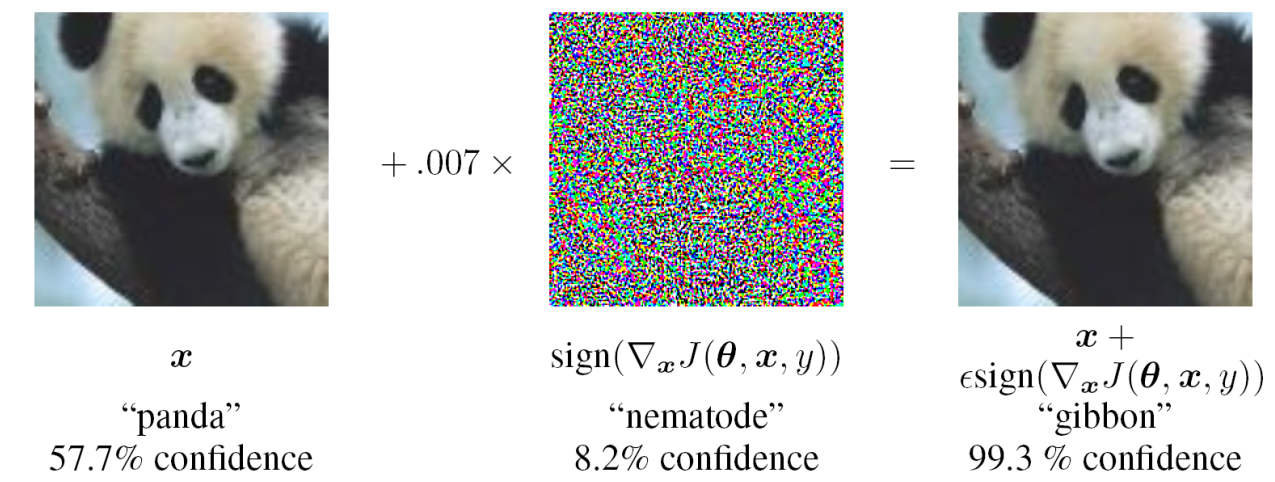
\includegraphics[width=0.9\textwidth,height=40mm]{images/panda_adversary.png}
    \caption{An adversarial example image generated by FGSM~\cite{goodfellow2014explaining}. The left side, a clean image of a panda, middle: the perturbation, right: the adversarial image classified as a gibbon}
    \label{fig:fgsm_example}
    \vspace{-4mm}
\end{figure}

\hspace*{3.5mm} Moreover, there is a close intersection between adversarial robustness and model interpretations~\cite{bhatt2020explainable,sharma2019certifai}. The closest adversarial example should perturb `fragile' features, enabling the model to fit to robust features, i.e., class-discriminating feature~\cite{bhatt2020explainable}. Often, discriminative models offer very limited performance guarantees when trained on data not generated by the same process as the training distribution, e.g., OOD~\cite{OOD1}. Further, the use of larger and more complex inputs in DL magnifies the difficulty of distinguishing between anomalous and in-distribution~(ID)~\cite{OOD5}. Such adversarial attacks are perhaps more critical in healthcare, especially when AI-guided systems is used to provide diagnosis help to the doctors, e.g., in the case of an OOD data point, a learning algorithm often encounter times not only makes a wrong or erroneous prediction but also can come up with a deadly error in clinical diagnosis~\cite{OOD1}. 

\hspace*{3.5mm} In the previous chapter, we have developed three models: a vanilla CNN, $MCAE_{slr}$, and $MCAE_{lrc}$ to predict cancer types based on patients genomics data. For the simplicity, imagine that we have a less complex CNN model trained on gene expression data. For the simplicity, we assume that the model shows 90\% confidence at predicting cancer types, when we evaluate on a sufficiently large test set. Once the model is deployed in our pipeline and ready for inferencing, we can make prediction for a single instance: given an image representation of a GE sample, the model predicts the cancer type as BRCA with 90\% probability. How confident are we that the input to our model is really a GE sample, not a CNV sample? In fact, the model will make a prediction. Making a wrong prediction is far better than a garbage prediction. We know through the adversarial attacks that in the presence of an adversary, we cannot trust blindly what our model says. Even if we assume there are no adversaries, we still would not have certainty that the input image is a GE sample. If we are given an independently sampled set generated or coming from the same distribution, the model is less likely to make wrong~(as well as garbage) prediction on more than a certain number of samples with a high probability.

\hspace*{3.5mm} Determining whether an input belongs to the population distribution of the training data, the model should be robust enough. In a larger extent, in order to ensure an explainable model is robust to adversaries and behaves as intended in real-life treatment diagnosis, we need to use adversarial training to improve performance. That is, if the sample is OOD, the predictions are unreliable, and the error cannot be bounded. Since we're emphasizing not only on high precision in clinical diagnosis, the model itself have to be able to detect OOD kind of adversaries, so that it is robust to such adversaries can lead to more human interpretable features by providing counterfactual explanations. 

\hspace*{3.5mm} In this chapter, we apply different types of adversarial attacks on our model, including  content moderation, numeric data moderation, and OOD, followed by assessing the robustness against these scenario. The rest of the chapter is structured as follows: \cref{chapter_6:rw} covers some related works on improving adversarial robustness of the machine learning models and summarize their potential limitations. \Cref{chapter_6:mm} describes the overall approach, including the detail of the data preparation before the network construction and training. \Cref{chapter_6:results} demonstrates the experiment results and discusses key findings of the study. Finally, \cref{chapter_6:conclusion} provides some explanations of the importance and relevance of the study reported, highlights the limitations and discuss some future works before concluding the chapter. 

\section{Related Work} \label{chapter_6:rw}
Since we apply content moderation (on numeric data) and OOD adversarial attacks, we limited our discussion on related work covering these two aspects only. Although some of the discussed works are not directly applicable for our cancer decision support system, they still provide the foundations to come up with effective adversarial robustness in our approach. Nevertheless, usually AEx are almost identical to normal samples, we treat attacks with AEx and OOD as two different types of attacks. 

\subsection{Attacks with adversarial examples}
Till date numerous approaches have been proposed on creating adversarial samples and some of them are already defeated by a countermeasure in later studies~\cite{yuan2019adversarial}. The concept of adversarial examples~(AEx) was first formulated by Dalvi et al.~\cite{dalvi2004adversarial} as a game between adversary and classifier in which the attack and defense on AEx can be correlate as an iterative game. One of the first gradient-based approaches was proposed to defend such adversary attack to generate AEx against linear SVM and a neural networks~\cite{biggio2013evasion}. However, Szegedy et al.\cite{szegedy2013intriguing} first introduced the concept of AEx against neural networks, where AEx were generated using a L-BFGS method\footnote{ Broyden–Fletcher–Goldfarb–Shanno is an iterative method for solving an unconstrained nonlinear optimization problem} as follows~\cite{yuan2019adversarial}:

\vspace{-6mm}
\begin{align}
    \begin{array}{cl}
        \min _{x^{\prime}} & c\|\eta\|+J_{\theta}\left(x^{\prime}, l^{\prime}\right) \\
         \text {s.t.} & x^{\prime} \in[0,1]
    \end{array}
    \label{eq:fgsm_aex}
\end{align}

\hspace*{3.5mm} where $c$ is a constant used to approximate values of AEx by linear-searching with $c > 0$, making it very expensive an expensive to find the optimal value for $c$. Subsequently, Goodfellow et al.\cite{goodfellow2014explaining}, proposed a fast method called Fast Gradient Sign Method~(FGSM) to generate AEx. The simplicity and effectiveness of FGSM relies on the fact that it needs to perform one step gradient update along the direction of the sign of gradient at each pixel, where the perturbation is expressed as~\cite{goodfellow2014explaining}: 

\vspace{-6mm}
\begin{align}
    \eta=\epsilon \operatorname{sign}\left(\nabla_{x} J_{\theta}(x, l)\right)
    \label{eq:fgsm_eta}
\end{align}

\hspace*{3.5mm} where $\epsilon$ is the magnitude of the perturbation, which is is computed using back-propagation. The corresponding adversarial example of sample $x$ is $x^{\prime}$, which is calculated as $x^{\prime}=x+\eta$~\cite{yuan2019adversarial}. On the other hand, literature~\cite{rozsa2016adversarial} proposed called called Fast Gradient Sign Method~(FGSM) to improve FGSM. In FGSM, the sign of gradient in FGSM is replaced with the raw gradient: $\eta=\nabla_{x} J(\theta, x, l)$. The effectiveness of FGSM relies in it's agnostic nature on constraints on each pixel, hence AEx can be generated with a larger local difference~\cite{yuan2019adversarial}. Since one-step attack is not only easy to transfer to another domain but also also easy to defend~\cite{yuan2019adversarial}, Dong. Y., et al.~\cite{dong2018boosting}, improve FGSM method in which momentum is applied to generate AEx more iteratively, where the gradients were calculated by:

\vspace{-6mm}
\begin{align}
    \mathbf{g}_{t+1}=\mu \mathbf{g}_{t}+\frac{\nabla_{x} J_{\theta}\left(x_{t}^{\prime}, l\right)}{\left\|\nabla_{x} J_{\theta}\left(x_{t}^{\prime}, l\right)\right\|},
\end{align}

\hspace*{3.5mm} AEx are then subsequently generated by   $x_{t+1}^{\prime}=x_{t}^{\prime}+ \epsilon sign g\_{t+1}$. A later method~\cite{tramer2017ensemble} proved that FGSM with adversarial training is more robust to white-box attacks than to black-box attacks due to gradient masking. RAND-FGSM is a new attack they proposed by adding random when updating the AEx to defeat adversarial training~\cite{yuan2019adversarial}:

\vspace{-6mm}
\begin{align}
    x_{t m p} &=x+\alpha \cdot \operatorname{sign}\left(\mathcal{N}\left(\mathbf{0}^{d}, \mathbf{I}^{d}\right)\right) \\
    x^{\prime} &=x_{t m p}+(\epsilon-\alpha) \cdot \operatorname{sign}\left(\nabla_{x_{t m p}} J\left(x_{t m p}, l\right)\right)
\end{align}
    
\hspace*{3.5mm} where $\alpha, \epsilon$ are the parameters, $\alpha<\epsilon$. On the other hand, DeepFool~\cite{moosavi2016deepfool} is another method to find the closest distance from the original input to the decision boundary of AEx. To overcome the non-linearity in high dimensional feature space, an iterative attack is performed with a linear approximation. Starting from an affine classifier~(AC), they found that the minimal perturbation of an AC is the distance to the separating affine hyperplane ${F}=\{x:$ $\left.w^{T} x+b=0\right\}$, where the perturbation of an AC, $F$ can be $\eta^{*}(x)=-\frac{F(x)}{\|w\|_{\text {is }}^{2}} w$~\cite{yuan2019adversarial}. In case of a binary differentiable classifier, $F$ an iterative method is employed to approximate the perturbation by considering $F$ is linearized around $x_{i}$ at each iteration, where the minimal perturbation is computed as follows:
 
\vspace{-6mm}
\begin{align}
    \begin{array}{ll}
    \underset{\eta_{i}}{\arg \min } & \left\|\eta_{i}\right\|_{2} \\
    \text {s.t.} & F\left(x_{i}\right)+\nabla F\left(x_{i}\right)^{T} \eta_{i}=0
    \end{array}
\end{align}

\hspace*{3.5mm} It is extended for multi-class classifier by finding the closest hyperplanes by finding a more general $\ell_{p}$ norm, $p \in[0, \infty)$. Eventually, DeepFool provides less perturbation compared to FGSM~\cite{yuan2019adversarial}.

\subsection{Attacks with OOD examples}
Subsequently, numerous approaches have been proposed to accurately identify OOD, in which many researchers have treated it as anomaly detection problem. Since discriminatively trained neural network classifiers produce reliable predictions only for ID samples, detecting OOD samples is essential. Assuming OOD to be outside the closed boundary of ID, typical neural classifiers do not contain the knowledge of this boundary for OOD detection during inference.  However, since OOD to be outside the closed boundary of ID, a predictive model is incapable of detecting OOD detection during the inferencing time. Subsequently, there have been several recent approaches to embed the logic into the learning algorithm and explicitly training the classifier with OOD samples close to the ID boundary. Oftentimes, the generated samples based on state-of-the-art approaches fail to cover the entire ID boundary effectively, thereby resulting in a sub-optimal OOD detector. 

\hspace*{3.5mm} Lee et al.~\cite{OOD13}, explains that test samples drawn sufficiently far away from the training distribution statistically or adversarially is a fundamental requirement for deploying a good classifier in many real-world machine learning applications. However, deep neural networks with the softmax classifier are known to produce highly overconfident posterior distributions even for such abnormal samples.  %Ensemble of Leave-Out Classifiers (ELOC
Jie et al.~\cite{OOD1}, proposed likelihood ratio method for deep generative models for OOD detection. Since the OOD is heavily affected by population level background statistics, they demonstrated that likelihood ratio method can effectively correct for these confounding back-ground statistics. Vernekar, Sachin et al.~\cite{OOD2} proposed of an efficient approach to generate OOD samples based on manifold learning network. OOD samples are used to train a classifier with an extra class~(i.e., $n+1$ classes, where ${(n+1)}^{th}$ class represents the OOD samples) for the detection of OOD during the inferencing time. They show that only a few OOD samples are sufficient to guide the decision boundary of the classifier to be bounded around the ID regions evidenced by their OOD detection results.

\iffalse
\begin{table}[h]
\centering
    \caption{Summary of recent related methods for OOD detection based on literature~\cite{OOD19}. Model update is how the method modifies the original classifiers. The benchmark results are based on DenseNet trained on CIFAR-100 as ID and TinyImageNet-resized as OOD. }
    \vspace{-2mm}
    \label{table:OODs_papers}
    \scriptsize
    \begin{tabular}{l|l|l|l|l|l} 
        \hline
        \textbf{Reference}  & \textbf{Method} & \textbf{Preprocessing require?} & \textbf{Model update} & \textbf{Data} & \textbf{AUROC} \\ \hline
        Qing Y. et al.~\cite{OOD19} & MDBC  & No & Fine tuning  & Labeled ID + unlabeled data  & 99.6 \\ \hline
        Liang Y. et al.~\cite{OOD13} & ODIN  & Yes & Static  & Labeled ID  & 90.7 \\ \hline
        Dan H. et al.~\cite{OOD18} & ODIN  & No & Static  & Labeled ID  & 71.6 \\ \hline
        Viyas A. et al.~\cite{OOD8} & ELOC  & Yes & Ensemble  & Labeled ID  & 96.3 \\ \hline
    \end{tabular}
\end{table}
\fi 

\hspace*{3.5mm} DeVries T. et al.~\cite{OOD3} shows that after training a DNN using IsoMax, ODD samples can be identified efficiently by simply calculating the entropy of the network's output probabilities. The approach proposed by them is called Entropic Score~(ES). The combined approach~(i.e., IsoMax for training and ES for ODD during inference) they proposed is also found to be fast, accurate, scalable, and unexposed. Based on the Outlier Exposure~(OE) technique, Rajati et al.~\cite{OOD4} proposed a novel loss function Outlier Exposure with Confidence Control~(OECC). They show that efficient optimization of OECC cam achieve state-of-the-art results in OOD detection with OE on both image and text classification tasks without needing much OOD samples. Vyas et al.~\cite{OOD8} proposed an ensemble method for the OOD detection which comprises of an ensemble of classifiers. Each classifier is trained in a self-supervised manner by leaving out a random subset of training data as OOD data and the rest as ID data. Although, sounds promising, the ensemble method based on randomly generated OOD samples mixed with real samples, did not preforms well, mainly because of in efficient way of generating OOD samples. 

\hspace*{3.5mm} Shalev et al.~\cite{OOD10}, proposed to use multiple semantic dense representations instead of sparse representation as the target label. Choi et al.~\cite{OOD11} proposed to scale OOD detection to high-dimensional data is to learn a tractable likelihood approximation of the training distribution, and use it to reject unlikely inputs. However, likelihood models on natural data are themselves susceptible to OOD errors, and even assign large likelihoods to samples from other datasets. Quintanilha  et al.~\cite{OOD12}, show that a simple ensembling of first and second order deep feature statistics can be exploited to effectively differentiate ID and OOD samples. It is observed that the mean and standard deviation within feature maps differs greatly between ID and OOD samples. Kliger et al.~\cite{OOD15} discuss the problem of simultaneous classification and novelty detection by determining whether an input is from the known set of classes and from which specific class, or from an unknown domain. They show a multi-class discriminator trained with a generator that generates samples from a mixture of nominal data distributions performs the best.

\hspace*{3.5mm} Liang et al.~\cite{OOD13} propose OOD image detection in neural networks~(ODIN), a simple and effective method that does not require any change to a pre-trained model. ODIN is based on the observation that using feature scaling and adding small perturbations to the input can separate the softmax score distributions between in- and OOD images, allowing for more effective detection. Based on experiments it is found that ODIN is compatible with diverse network architectures and datasets. Hendrycks et al.~\cite{OOD17} considers two related problems of detecting if an example is misclassified or OOD. A simple baseline that utilizes probabilities from softmax distributions can be found effective in computer vision, NLP, and automatic speech recognition. In a later approach, Qing et al.~\cite{OOD19} propose a two-head deep CNN architectures and maximize the discrepancy between the two classifiers~(MDBC) to detect OOD inputs. It train a two-head CNN consisting of one common feature extractor and two classifiers which have different decision boundaries but can classify ID samples correctly. 

\iffalse
\begin{table*}[!ht]
    \caption{different cancer detection methods, data types, and performance }
    \label{table:stateofart}
    \begin{center}
    \scriptsize
    \vspace{-6mm}
    \begin{tabular}{l|l|l|l}
        \hline
        \textbf{Reference} & \textbf{Approach} & \textbf{Use cases} & \textbf{AUROC/FPR} \\\hline
            Ren, Jie et al.~\cite{OOD1} & Likelihood ratios & Imaging \& genomics & 93\%/6.6\% \\\hline % 2018
            Vernekar, Sachin et al.~\cite{OOD2} & Manifold learning network & MNIST and Fashion-MNIST classification & 99.6\%/0.4\% \\\hline % 2018
            DeVries, Terrance et al.~\cite{OOD3} & Learning confidence estimates & Imaging & 99.1\%/9.3\% \\\hline % 2018
        	Papadopoulos, Rajati et al.~\cite{OOD4} & Confidence control & Image \& texts  & 97.81\%/6.1\%  \\\hline  % 2017
            Dan, Hendrycks et al.~\cite{OOD5} &  Outlier exposure & Imaging & 89.3\%/9.5\% \\\hline % 2016
            M. Masana et al.~\cite{OOD6} & Metric learning  & MNIST and SVHN & 75\% \\\hline % 2016
        	Rajana et al.~\cite{20Rajanna} & Deep NN & Prostate cancer & 95\%\\\hline
            Chen et al.~\cite{18Chen} & Shallow NN & Colon cancer  & 84\% \\ \hline % 2015
            Ahmed et al.~\cite{abdel2016breast} & DBN & Breast cancer  & 99\% \\ \hline % 2015
            Zheng et al.~\cite{23Zheng} & K-means/SVM & Breast cancer & 97.38\% \\ \hline % 2014
            Xiaofan et al.~\cite{ding2014application} & Naïve Bayes & Cancer risk & 93\% \\ \hline % 2014
        \end{tabular}
    \end{center}
\end{table*}
\fi 

\section{Methods}\label{chapter_6:mm}
In this section, we cover different threat models for different types of adversarial attack. Depending upon scenarios, assumptions, and quality requirements of diagnosis, we then generate AEx to deploy specific attack approaches, followed by adversary training to defend the adversary attacks. 

\subsection{Formulating threat models}
Literature~\cite{yuan2019adversarial}, decomposed the threat models into 4 different aspects: i) adversarial falsification (i.e., in which negative and positive sample are generated with false positive and false negative attacks, respectively), adversary's knowledge~(e.g., depending upon if the deployed model is a white-box or a black-box model), adversarial specificity~(e.g., targeted or non-targeted attacks), and attack frequency~(i.e., one-time or iterative attacks). In a white-box attack scenario, it is assumed that the adversary has sufficient knowledge about the model, including the training data, model architectures, hyper-parameters, numbers of layers, activation functions, and model weights~\cite{yuan2019adversarial}. In order to perform the attack, AEx are generated by calculating model gradients. 

\hspace*{3.5mm} On the other hand, a black-box attack assumes that the adversary has no access to (or knowledge about) the trained model, but knows what the model is for, e.g., knows the output~(e.g., confidence score) of the model. Although, most attacks with AEx are white-box attacks, they can be applied to black-box attacks due to the transferability of AEx~\cite{papernot2016transferability}. Targeted attacks misguide a trained model to a specific class, which is usually occur in the multiclass classification problem. For example, an adversary fools our cancer types classifier to predict all AEx of breast cancer. Targeted attacks usually maximize the probability of targeted adversarial class~\cite{yuan2019adversarial}. A non-targeted attack does not assign a specific class to the network's output. Hence, the class output can be arbitrary, except the original one.

\begin{figure}[htp!]
    \centering
    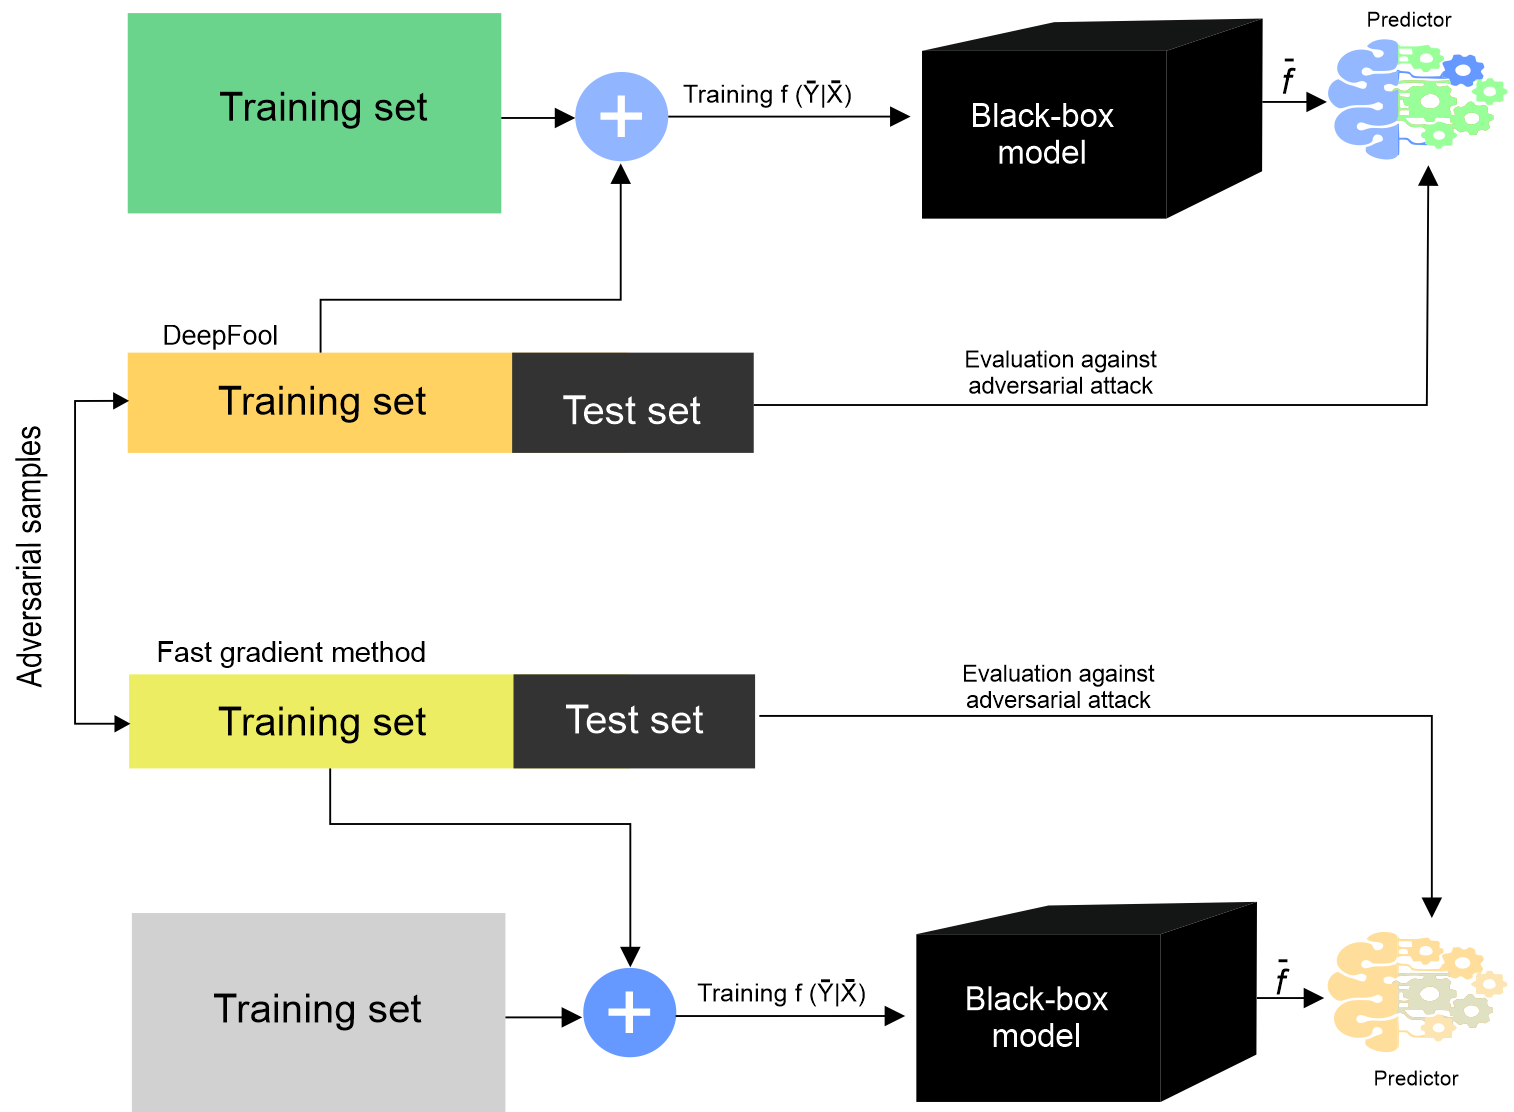
\includegraphics[width=0.7\textwidth,height=60mm]{images/aattacks.png}
    \caption{Two types of attack scenarios: up: minor content moderation across samples with fast gradient sign method~\cite{goodfellow2014explaining}, below: crafting adversarial samples with DeepFool}
    \label{fig:aattacks}
    \vspace{-2mm}
\end{figure}

\iffalse
\begin{figure}[htp!]
    \centering
    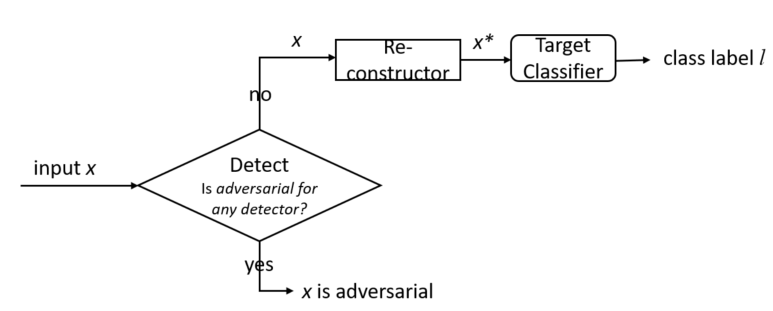
\includegraphics[width=0.8\textwidth,height=50mm]{images/robustness_wf.png}
    \caption{Workflow of the methods}
    \label{fig:robustness_workflow}
\end{figure}
\fi 

\hspace*{3.5mm} Since non-targeted attacks are easier to implement compared to targeted attacks, and keeping in mind the scope of this thesis, we performed non-targeted attacks in a black-box scenario only. We apply two types of adversarial attacks on our models: i) attack with AEx generated content moderation attack, ii) attack with AEx generated with DeepFool. %, iii) attack with OOD samples generated with GAN. %The first two attacks falls in the content moderation attack category. 
AEx are expected to be close to the original samples and should be imperceptible to a human, which causes the performance degradation of any ML models compared to that of a human~\cite{goodfellow2014explaining}. Nevertheless, the same adversarial example is often misclassified by a variety of classifiers with different architectures or trained on different subsets of the training data~\cite{yuan2019adversarial,goodfellow2014explaining}. We hypothesize that a black-box model with adversarial robustness capability, will still be able to generate moderately fair and reliable explanations. 

\subsection{Adversarial attacks}
%Before a model is deployed, robustness needs to be improved to improve content detection accuracy under the adversarial attack. 
For each target model, we generate AEx from test samples as outlined in \Cref{fig:aattacks} and use only those that can attack successfully before deploying any counter measure in all of our experiments. 
%\subsubsection{Adding Gaussian noises}
%\subsubsection{Adversarial samples generation}
%The linear view of adversarial examples suggests a fast way of generatingthem.%Since neural networks are too linear to resist linear adversarial perturbations. More nonlinear models such as Sigmoid networks are carefully tuned to spend most of their time in the non-saturating, more linear regime for the same reason. This linear behavior suggests that cheap, analytical perturbations of a linear model should also damage neural networks. 
We introduce two types of attack scenarios in which samples AEx are generated: i) with content moderation across samples, ii) crafting AEx with DeepFool.
%, iii) with GAN-based approach. 
For the first one, we employed the FGSM to generate AEx with content moderation, where the gradient is computed using backpropagation. For a given trained model $F$ and an original input data sample $x$, generating an adversarial example $x^{\prime}$ can be formulated as a box-constrained optimization problem~\cite{yuan2019adversarial}:

\vspace{-6mm}
\begin{align}
    \begin{array}{cl}
        \min _{x^{\prime}} & \left\|x^{\prime}-x\right\| \\
        \text {s.t.} & F\left(x^{\prime}\right)=y^{\prime} \\
        & F(x)=y \\
        & l \neq y^{\prime} \\
        & x^{\prime} \in[0,1],
    \end{array}
\end{align}

where $y$ and $y^{\prime}$ is the predicted label of $x$ and $x^{\prime},\|\cdot\|$ is the distance between two samples. 

\hspace*{3.5mm}Let $\eta=x^{\prime}-x$ be the perturbation added on $x$ and minimizes the perturbation while misclassifying the prediction with a constraint of input data, ${\theta}$ is the model parameter, ${x}$ is the input, $y$ targets associated with ${x}$ and $J( \theta, x,y)$ is the cost used to train a DNN architecture. The cost function around the current value of ${\theta}$ can be linearize by obtaining an optimal max-norm constrained perturbation as outlined in \cref{eq:fgsm_eta}. To craft AEx, we employ an iterative optimization-based approach called DeepFool, which has higher success rates under the same norm objective in a white-box setting~\cite{yuan2019adversarial}. Since DeepFool provides less perturbation compared to FGSM~\cite{yuan2019adversarial}, we consider  AEx generated with FGSM as OOD attack. 

%\subsubsection{Attack with crafted adversarial samples}
%\subsection{OOD attacks}
\iffalse
We generated OOD samples
%~(equal number of samples used to train MCAE classifiers) 
using `Natural GAN'~(NGAN)\footnote{\url{https://github.com/zhengliz/natural-adversary}}~\cite{zhao2017generating}. 
GAN-based AEx are more natural to human. First, we train a Wasserstein GAN model on the PCAt datasets, where the generator $\mathcal{G}$ maps random noise to the input domain. Additionally, we train an ``inverter" $\mathcal{I}$ to map input data to dense inner representations, where adversarial noise is generated by minimizing the distance of the inner representations. AEx were generated using the generator $  x^{\prime}=\mathcal{G}\left(z^{\prime}\right)$, where~\cite{OOD19,zhao2017generating}: 

\vspace{-6mm}
\begin{align}
    \begin{array}{cl}
        \min _{z} & \|z-\mathcal{I}(x)\| \\
        \text {s.t.} & f(\mathcal{G}(z)) \neq f(x)
    \end{array}
\end{align}

\hspace*{3.5mm}Both the generator $\mathcal{G}$ and the inverter $\mathcal{I}$ were built to make adversarial examples natural. Another reason of using NGAN in the black-box attack scenario that it does not require gradients of original neural networks. The GAN-based data generation workflow is shown in \cref{fig:OOD_GAN_generation}. 

\begin{figure*}
	\centering
	\begin{subfigure}{.61\linewidth}
		\centering
		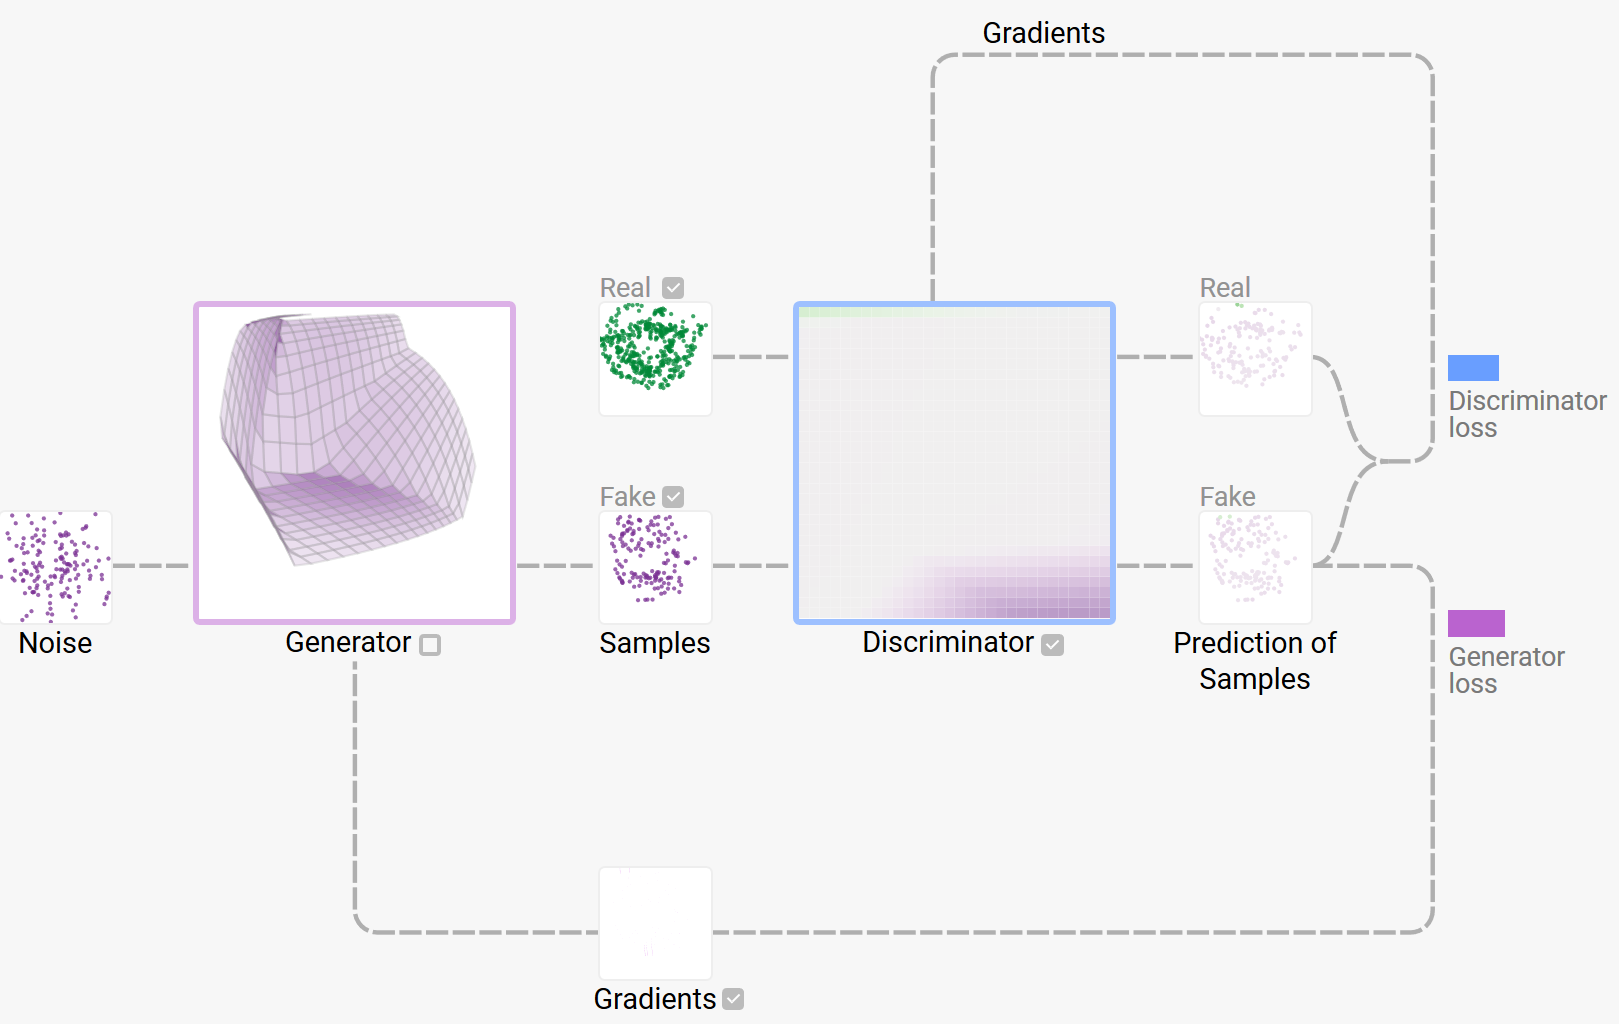
\includegraphics[width=\linewidth,height=60mm]{images/gan_sg.png}
		\caption{OOD sample generation}
        \label{fig:ood_sample-generation}
	\end{subfigure}
	\begin{subfigure}{0.35\linewidth}
		\centering
		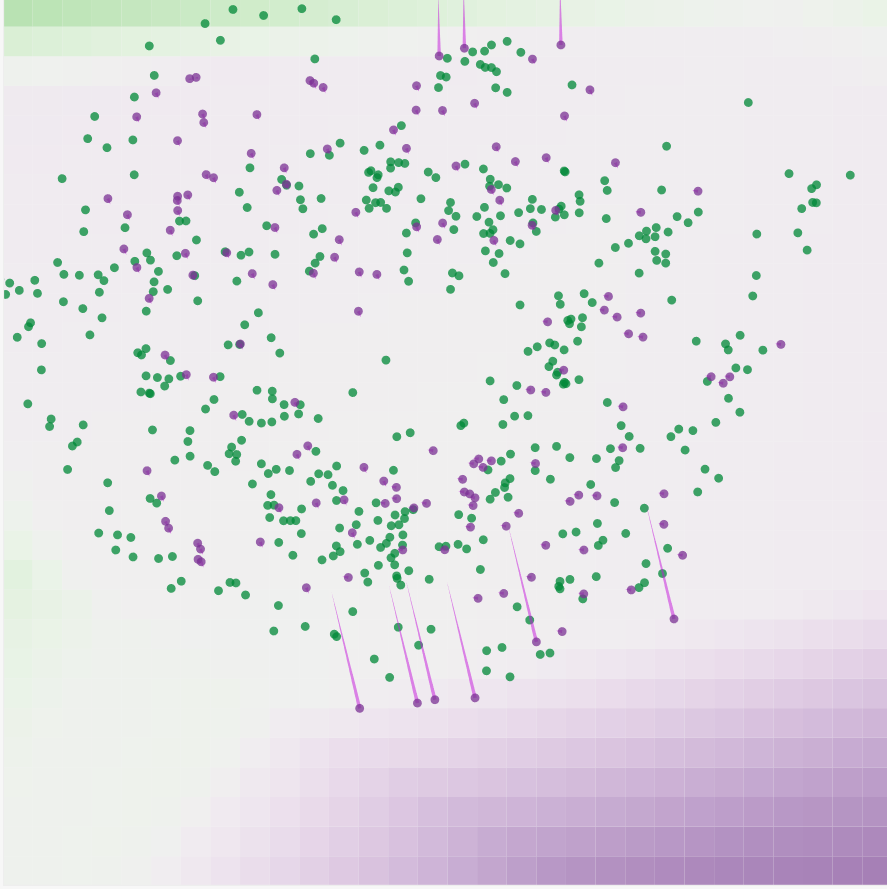
\includegraphics[width=\linewidth,height=60mm]{images/ld.png}
		\caption{Layered distribution}
	\end{subfigure}
	\caption{GAN-based OOD sample generation: green \& purple dots represent real and fake samples~\cite{kahng2018gan}} 
	\label{fig:OOD_GAN_generation}
\end{figure*}
\fi 

\subsection{Defenses against attacks}
Literature~\cite{OOD19} has outlined two types of countermeasures against adversarial attacks called `reactive' and `proactive'. The former deals with detecting AEx after a ML model is trained. Examples include adversarial detecting, input reconstruction, and network verification. The latter deals with by making a ML more robust before an adversary generates and attacks with AEx. Examples include network distillation, adversarial (re)training, and classifier robustifying. However, keeping in mind the scope of this thesis, we try to impose a light weight countermeasures. 

\begin{figure}[htp!]
    \centering
    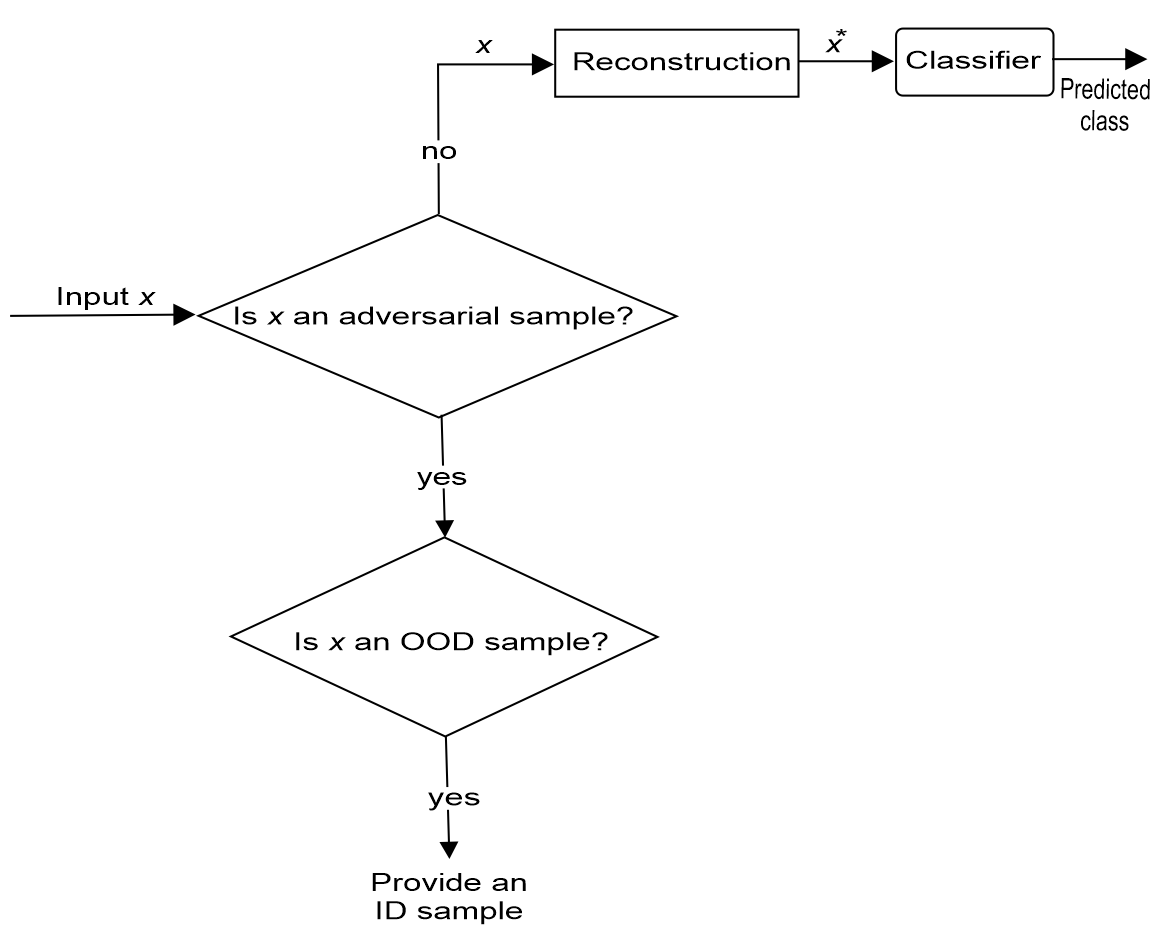
\includegraphics[width=0.7\textwidth,height=90mm]{images/reactive_measure.png}
    \caption{Workflow of reactive measures against an adversarial sample during the inferencing}
    \label{fig:reactive_measures}
    \vspace{-4mm}
\end{figure}

\subsubsection{Proactive measure: adversarial retraining}
We evaluate the models on adversarial test examples, before employing any defense. Given two different gradient-based cancer type~i.e., trained) classifiers $F_1$ and $F_2$~(e.g., $MCAE_{slr}$ and $MCAE_{lrc}$ models trained on the multimodal genomics data based on shared latent representation and latent representation concatenation, respectively), the robustness of each content moderation model is measured by the minimum perturbations required for an input sample to evade detection. For model $F: \mathbb{R}^{D} \rightarrow$ $\{1, \ldots, K\}$~(either $F_1$ or $F_2$), assuming $F(x)=\operatorname{argmax}_{i}\left(Z(x)_{i}\right)$, where $Z(x) \in\mathbb{R}^{K}$ is the final layer output, and $Z(x)_{i}$ is the prediction score for the $i^{th}$ class. Similar to literature~\cite{bhatt2020explainable}, we then formulate the objective w.r.t. to find the minimum perturbation~\cite{bhatt2020explainable} as an optimization problem formulated as follows:

\vspace{-6mm}
\begin{align}
    \underset{\boldsymbol{x}}{\operatorname{argmin}}\left\{d\left(\boldsymbol{x}, \boldsymbol{x}_{0}\right)+c {L}(\boldsymbol{f}(\boldsymbol{x}), y)\right\},
\end{align}

where $d(\cdot, \cdot)$ is a distance measure $\ell_{2}$~(i.e., Euclidean distance), ${L}(\cdot)$ is the `cross-entropy loss~(CEL)' function and $c$ is a balancing factor. However, searching for possible AEx is an expensive and non-trivial problem. The projected gradient descent~(PGD) is a commonly used method, which search for the minimum perturbation from the test set of allowable perturbations ${S} \subseteq \mathbb{R}^{D}$ as follows~\cite{bhatt2020explainable}: 

\vspace{-6mm}
\begin{align}
    x^{t+1}=\Pi_{x+\mathcal{S}}\left(x^{t}+\alpha \operatorname{sgn}\left(\nabla_{x} \mathcal{L}\left(f_{\theta^{*}}(x), y\right)\right)\right),
    \label{eq:search_perbu}
\end{align}

\hspace*{3.5mm}\cref{{eq:search_perbu}} holds until $x^{t}$ is misclassified by the model successfully. Based on the $\ell_{2}$-norm perturbation distance averaged over $n$ test samples: the larger the average perturbation, the more robust the model is, as it takes greater effort for an attacker to evade detection~\cite{bhatt2020explainable,yuan2019adversarial}. 
%The average perturbation required is also widely used as a metric when comparing different candidate models and different versions of a given model. 
Therefore, more robust models have more convincing gradient-based explanations, i.e., the gradient of the output w.r.t the input shows that the model is focusing on relevant portions of an input object~(e.g., image)~\cite{bhatt2020explainable}.

\subsubsection{Reactive measure: input reconstruction}
Now let's assume, we identified AEx with minor content moderation. Therefore, we can also assume that because of different data generation platform~(e.g., human methylation 450K vs. 27K), an adversarial sample is slightly different than a original sample. Based on this assumption, we attempted to still make a meaningful prediction by correcting or reconstructing a clean representation. Nevertheless, AEx can be transformed to corresponding clean input via reconstruction. After the transformation, an adversarial sample will not be able to affect the prediction of a trained model~(at least not that severely). 
To increase the robustness of DNNs, deep contractive autoencoder is proposed by introducing penalty~\cite{meng2017magnet}, were a denoising AE~(DAE) is trained to encode AEx to original ones to remove adversarial perturbations. 

\hspace*{3.5mm} As stated in \cref{chapter:introduction}, noise can be introduced to the input~\cite{min2018survey} to improve the robustness of the representation learning~(RL), followed by the extraction of composing robust features\footnote{We already introduced noise via Gaussian noise layers to make the snapshot models~(refer to \cref{chapter:uni_modality}) learn little variations, which helped both Conv-LSTM and CAE classifiers improve the generalization. }. Hence reconstruction of the AEx is possible by adding Gaussian noise~\cite{OOD19}. First, to simulate the scenario, we added Gaussian noises to features in the GE, miRNA, and CNV data with zero mean and standard deviations of 0-200\% $(k)$ of $i^{\text {th}}$ per feature~(i.e., gene) average $\left(\mu_{i}\right),$ or $N(0, k \mu)$ per feature. We apply PixelCNN proposed in PixelDefend~\cite{song2017pixeldefend} to reconstruct the AEx back to the training distribution, where all pixels are changed along each channel to maximize the probability distribution~\cite{song2017pixeldefend}:

\vspace{-6mm}
\begin{align}
    \begin{array}{cl}
        \max _{x^{\prime}} & {P}_{t}\left(x^{\prime}\right) \\
        \text {s.t.} & \left\|x^{\prime}-x\right\|_{\infty} \leq \epsilon_{\text {defend}}
    \end{array}
\end{align}

\hspace*{3.5mm} where ${P}_{t}$ denotes the training distribution, $\epsilon_{\text {defend}}$ controls the new changes to AEx. For a supplied input~(i.e., perturbed sample) $x^{\prime}$, first we reconstruct a cleaner version $x^c$ using PixelCNN, which we use to classify into a specific cancer type using model $F: {X}^{(m)} \rightarrow {Y}$~(e.g., either $F_1$ or $F_2$ for multimodal inputs and CNN for unimodal input), where predictor $F$ maps instance $x$ from a feature space ${X}^{(m)}$ with $m$ input features to a labels $y$ in a target space ${Y}$, where $F(x)=y$ denotes the decision $y$, predicted by $F$. %Further, we employ PixelDefend for the detection of possible AEx, i.e, if an adversarial example . 

\subsubsection{Reactive measure: out-of-distributions detection}
\noindent The prediction probability of OOD samples tends to be lower than the prediction probability of ID samples~\cite{OOD18}. Therefore, OOD samples are closer to the class boundaries and more likely to be misclassified~(or classified with low confidence) by a classifier trained on ID samples. In our approach, to mitigate OOD issue, the likelihood ratio is calculated for the OOD samples before inferencing to avoid such instance.  
%Inspired by literature~\cite{OOD1}, we trained a variational autoencoder~(VAE) on gene expression dataset for OOD detection by employing a method called likelihood ratio to observe the effects of likelihood score by population level background statistics. %We demonstrate the generality of the proposed method by showing that it significantly improves OOD detection when applied to deep generative models of images. 

%\paragraph{Problem formulation}
We assume that an ID~(sample, label) pair, $\left\{\mathrm{x}_{\text {in}}, y_{in}\right\}$ drawn from a set of labeled ID samples $\left\{X_{in}, Y_{in}\right\}$ and $\mathbf{x}_{\mathbf{ul}}$ is drawn from unlabeled samples, and $\mathrm{x}_\text{in} \in \left\{\mathrm{x}_{\text {ge}}, \mathrm{x}_{\text {mr}}, \mathrm{x}_{\text {cnv}}\right\}$, when all the individual modalities are considered. The ID sample $\left\{\mathbf{x}_{\text {in}}, y_{in}\right\}$ can be classified into $K$ classes, i.e., $y_{in} \in K$, and $\mathbf{x}_{\mathbf{ul}}$ can be either an ID or an OOD samples, where $\exists\left\{\mathbf{x}_{\text {ul}}, y_{ul}\right\}, y_{ul} \notin K$. Since the goal is to distinguish whether a sample $\mathbf{x}_{\mathbf{ul}}$ is from ID or OOD, we train the network to predict different softmax class probabilities for ID samples and OOD samples by utilizing $\mathbf{x}_{\mathbf{u}1}$ during the unsupervised training as literature~\cite{OOD19}. 

\begin{figure}
    \centering
    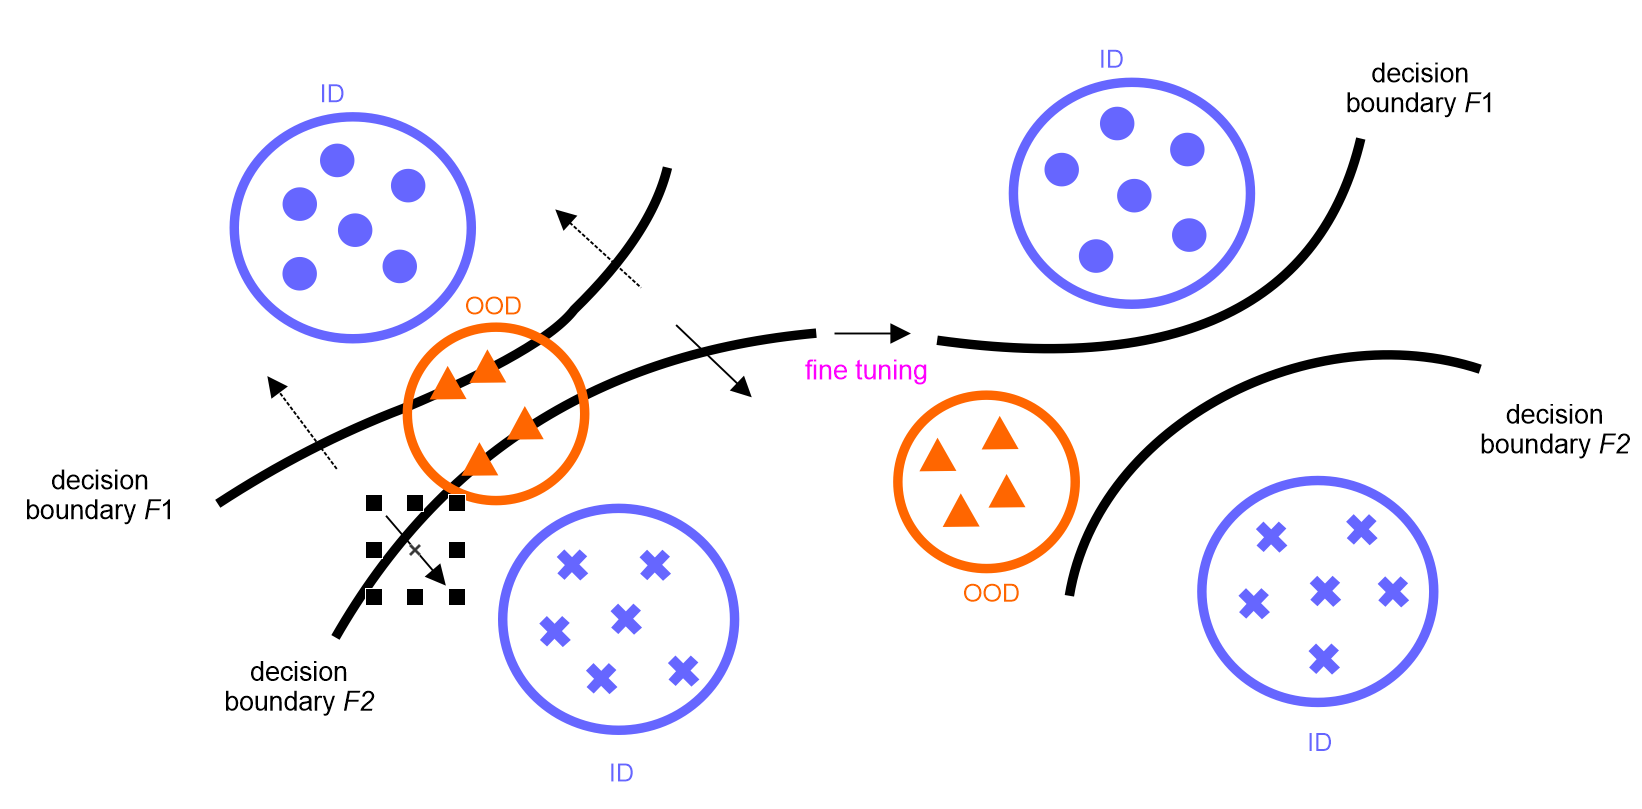
\includegraphics[width=0.7\textwidth,height=60mm]{images/ood_ex_1.png}
    \caption{Detection of OOD samples by the discrepancy between two classifiers based on~\cite{OOD19}, where $MCAE_{slr}$ and $MCAE_{lrc}$ represent model $F_1$ and $F_2$, respectively}
    \label{fig:ood_detection_example}
    \vspace{-4mm}
\end{figure}

\hspace*{3.5mm} From a given ID dataset ${D}$ of $(\boldsymbol{x}, y)$ pairs sampled from the distribution $p^{*}(\boldsymbol{x}, y)$ where $x$ is the extracted feature vector or raw input and $y \in {Y}:=\{1, \ldots, k, \ldots, K\}$ is the label assigning membership to one of $K$ ID classes. In the corresponding profiles~(i.e., GE, miRNA, or CNV), inputs are numeric or discrete, i.e. $x_{d} \in \mathbb{R}$. In general, OOD inputs are sampled $(\boldsymbol{x}, y)$ generated from an underlying distribution other than $p^{*}(\boldsymbol{x}, y)$. Similar to literature~\cite{OOD1}, we then consider an input $(x, y)$ to be OOD if $y \notin {Y}$, i.e., the class $y$ does not belong to any of $K$ ID classes. This turns out the OOD detection is a task to accurately detect if an input $x$ is OOD or not~\cite{OOD1,OOD2,OOD3}.

%\paragraph{Network constructions}
\hspace*{3.5mm} Similar to literature~\cite{yu2019unsupervised}, we construct a two-head neural network architectures consisting of a feature extractor, $E,$ which takes inputs $\mathrm{x}_{\text {in }}$ or $\mathrm{x}_{\mathrm{ul}}$, and two classifier $F_{1}$ and $F_{2}$, where each classifier takes features from $E$ and predict into one of $K$ classes. Classifiers $F_{1}$ and $F_{2}$ output a $K$ dimensional vector of logits. The class probabilities is then calculated using softmax activation, where $p_{1}(\mathbf{y} | \mathbf{x})$ and $p_{2}(\mathbf{y} | \mathbf{x})$ are $K$ dimensional softmax class probabilities for input $x$ produced with classifier $F_{1}$ and $F_{2}$, respectively. In our case, we assume each sample consisting of 3 different modalities, i.e., gene expression, copy numbers, and miRNA expression, s.t., we create latent representation of each input modality as shown in \cref{fig:ood_network}. 

\begin{figure}[htp!]
    \centering
    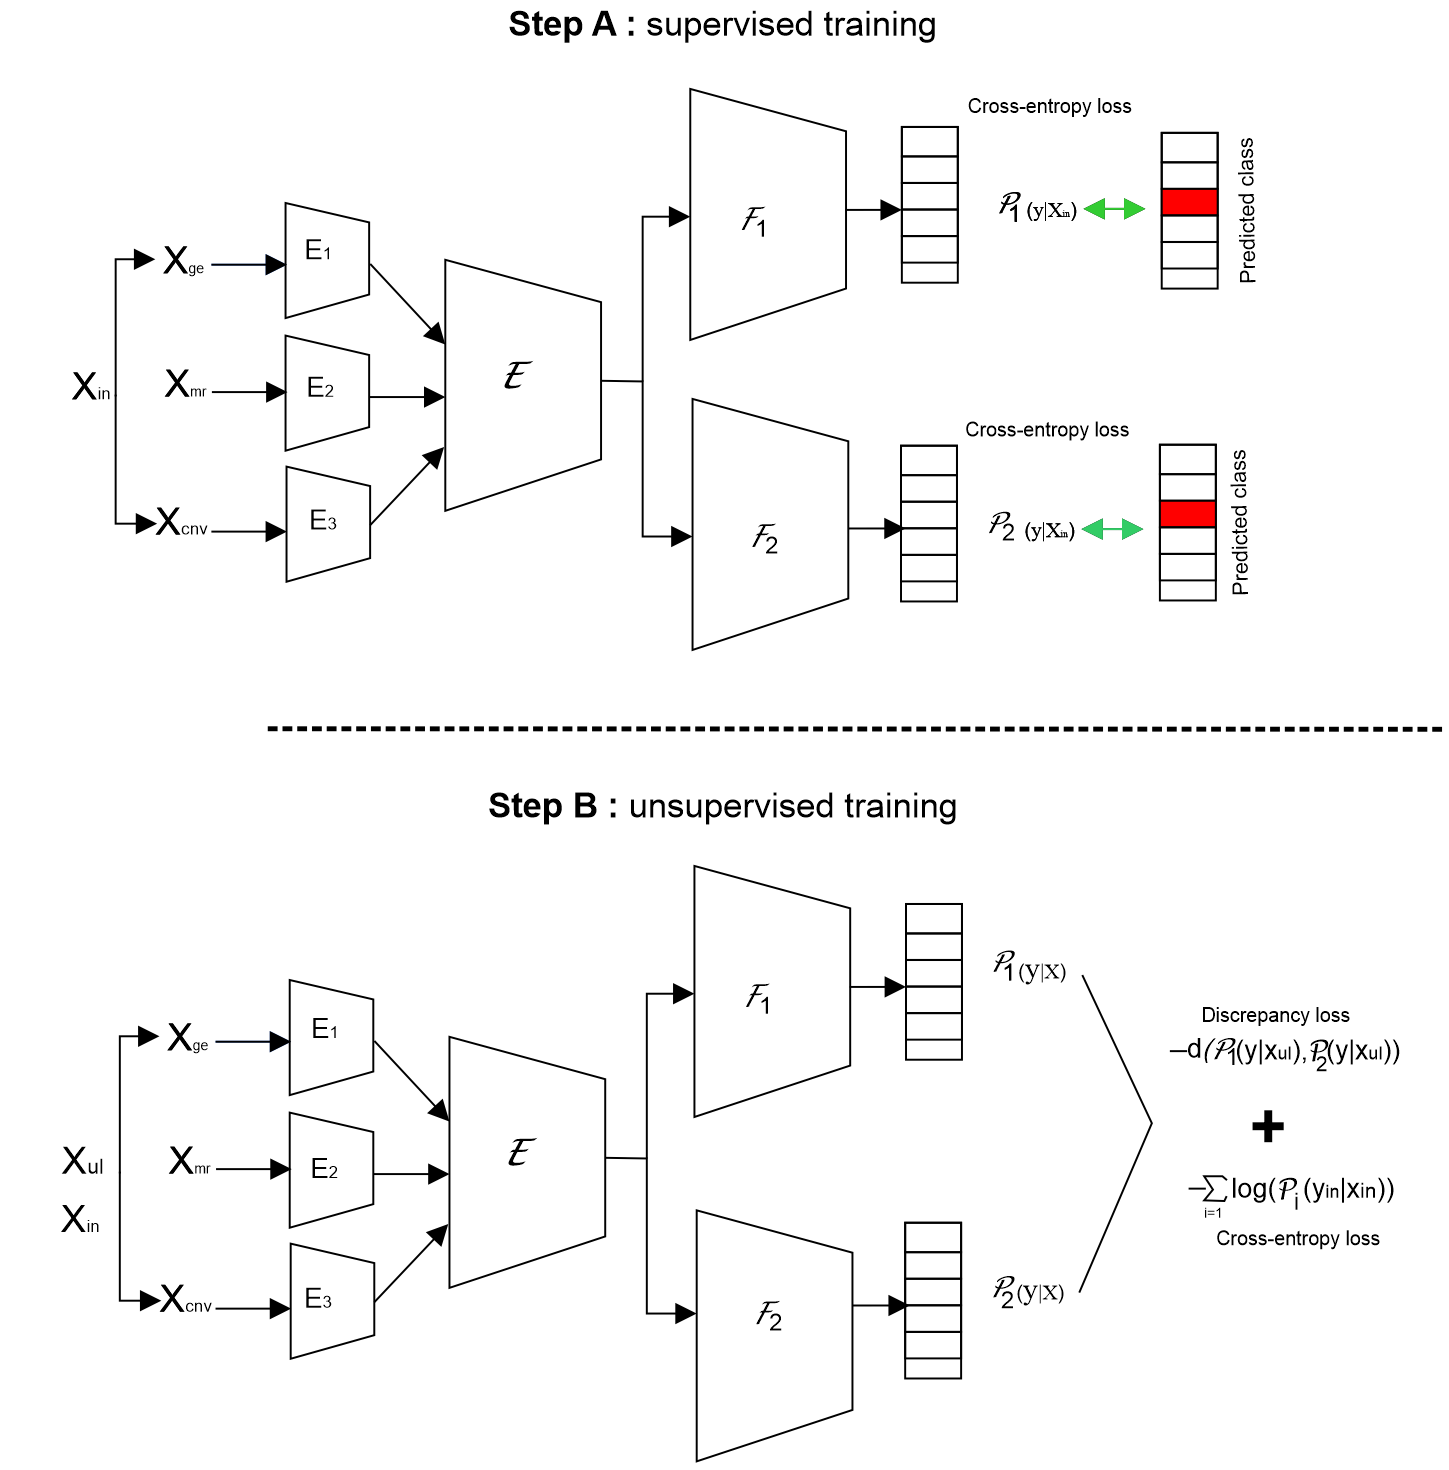
\includegraphics[width=0.8\textwidth,height=100mm]{images/OOD_1.png}
    \caption{Supervised pre-training and unsupervised fine-tuning steps for OOD detection method which we extended for multimodal scenario is based on~\cite{yu2019unsupervised}. The network consists of an extractor $E$ and two classifiers $F_{1}$ and $F_{2}$. \textbf{Step A}: supervised training to classify ID samples correctly. \textbf{Step B}: $F_{1}$ and $F_{2}$ learn to maximize the discrepancy in an unsupervised manner to detect OOD samples}
    \label{fig:ood_network}
    \vspace{-2mm}
\end{figure}

\hspace*{3.5mm} If two different classifiers~(i.e. $F_{1}$ and $F_{2}$ in our case) are initialized with random initial parameters and subsequently trained on ID samples supervised way, they are tend to show slightly different characteristics. Nevertheless, most OOD samples have larger discrepancy than ID samples, two different classifiers classify OOD samples differently~\cite{OOD19}. 
%Based on the characteristic of OOD samples,  
We measure the disagreement between the classifiers and train the network to maximize it. Similar to literature~\cite{OOD19} we hope that the network will push OOD samples outside the manifold of ID samples. Consequently, OOD samples and ID samples can be separated according to the discrepancy between the two classifiers’ outputs as shown in \cref{fig:ood_detection_example}, where discrepancy loss is computed as follows to measure the divergence between the two softmax class probabilities for an input~\cite{OOD19}: 

\vspace{-6mm}
\begin{align}
    d\left(p_{1}(\mathbf{y} | \mathbf{x}), p_{2}(\mathbf{y} | \mathbf{x})\right)=H\left(p_{1}(\mathbf{y} | \mathbf{x})\right)-H\left(p_{2}(\mathbf{y} | \mathbf{x})\right)
    \label{eq:dis_loss_1}
\end{align}

\noindent where $H(\cdot)$ is the entropy over the softmax distribution. Again similar to literature~\cite{yu2019unsupervised}, the whole training consists of supervised pre-training and unsupervised fine-tuning. During the pre-training, we train the network to learn discriminative features before classifying the ID samples correctly in a supervised way. Since this is a supervised way to predict the labels, we optimize the following CEL~\cite{yu2019unsupervised}:

\vspace{-6mm}
\begin{align}
    {L}_{sup}=-\frac{1}{\left|X_{i n}\right|} \sum_{\mathbf{x}_{\mathrm{in}} \in X_{i n}} \sum_{i=1}^{2} \log \left(p_{i}\left(y_{i n} | \mathbf{x}_{\mathrm{in}}\right)\right)
\end{align}

\hspace*{3.5mm} Once the network converges, we perform unsupervised fine-tuning to increase the discrepancy in an unsupervised manner in order to make the network detect the OOD samples that do not have the support of the ID samples. During the supervised learning, we keep training the network to classify the labeled ID samples by minimizing the CEL to maintain the manifold of ID samples. To optimize both supervised and unsupervised losses, we first combine them and optimize jointly similar to literature~\cite{yu2019unsupervised}: 

\vspace{-4mm}
\begin{align}
    \begin{array}{c}
        {L}={L}_{sup}+{L}_{unsup} \\ 
        {L}_{sup}=-\frac{1}{\left|X_{i n}\right|} \sum_{\mathbf{x}_{\mathrm{in}} \in X_{in}} \sum_{i=1}^{2} \log \left(p_{i}\left(y_{i n} | \mathbf{x}_{\mathrm{in}}\right)\right) \\ 
        {L}_{unsup}=\max \left(m-\frac{\sum_{\mathbf{x}_{\mathbf{u} 1} \in X_{ul}} d\left(p_{1}\left(\mathbf{y} | \mathbf{x}_{\mathbf{ul}}\right), p_{2}\left(\mathbf{y} | \mathbf{x}_{\mathbf{ul}}\right)\right)} {\left|X_{ul}\right|},0\right)
    \end{array}
    \label{eq:ood_join_loss}
\end{align}

\hspace*{3.5mm} where, $m$ is the margin used to prevent overfitting, i.e., if the average discrepancy of unlabeled samples is greater than the margin m, the unsupervised loss will equal its minimum value zero~\cite{yu2019unsupervised}. Since the network is already trained to maximize the discrepancy loss, which means the the entropy of $F_1$’s output is tend to be maximized and the entropy of $F_2$’s output to get minimized. Consequently, $F_2$ is expected to predict high probability of one class. In that case, OOD samples will be outside the support of the ID samples making the discrepancy between the outputs of $F_{1}$ and $F_{2}$ for OOD samples to be larger. During the inference time, in order to distinguish between ID and OOD samples, similar to literature~\cite{yu2019unsupervised}, the discrepancy is computed w.r.t, the $L_1$ distance between $F_{1}$ and $F_{2}$ classifier's outputs. When the distance is above a detection threshold $\delta$, we consider the sample as an OOD sample denoted as follows~\cite{yu2019unsupervised}: 

\vspace{-6mm}
\begin{align}
    \sum_{i=1}^{K}\left|p_{1}\left(y_{i} | \mathbf{x}\right)-p_{2}\left(y_{i} | \mathbf{x}\right)\right|>\delta, 
\end{align}

where $x$ could be a unimodal or multimodal sample. Subsequently, we stop making the inferencing for an OOD samples, given that making a wrong prediction is far better than a garbage prediction. 
\section{Experiments}\label{chapter_6:results} 
In this section, we discuss the evaluation results of content moderation attack and OOD detection, both quantitatively and qualitatively. %Besides, a comparative analysis with state-of-the-art approaches is provided. 

\subsection{Experiment setup}
%All the programs were written in Python\footnote{\url{https://github.com/rezacsedu/XAI_Cancer_Prediction}}. The software stack consists of scikit-learn and Keras with TensorFlow backend. The network was trained on an Nvidia GTX 1080i GPU with CUDA and cuDNN enabled to make the overall pipeline faster. 
%Further, since an appropriate selection of hyperparameters can have a huge impact on the performance of a deep architecture, we perform the hyperparameter optimization through a random search and 5-fold cross-validation tests. In each of 5 runs, 70\% of the data is used for the training, 30\% for the evaluation, while 10\% of the training set is used for validation of the networks to optimize the cross-entropy loss based on the best learning rate, batch size, number of filters, kernel size, and dropout/Gaussian noise probability. 
%\subsubsection{Setup for content moderation detection}
%\subsubsection{Setup for OOD detection}
For the pre-training, we follow steps similar to literature~\cite{OOD19}, but using Adam optimizer to train both MCAE classifiers for 200 epochs. The learning rate~(LR) started at 0.1 and dropped by a factor of 10 at 50\% and 75\% of the training progress, respectively. During the fine-tune, we iterate each fit for 50 epochs, by setting margin m = 1:2 to detect OOD samples. Subsequently, we select the best classifier using WeightWatcher. %Results based on hyperparameters produced through random search and 5-fold cross-validation are reported and discussed with a comparative analysis with AUROC, AUPR, FPR, TPR, FNR, and DE. 
To assess the robustness of our models, we compute the empirical robustness metric~(ERM) of a classifier object over the test set for a given adversarial crafting method attack as suggested in literature~\cite{moosavi2016deepfool}. The ERM is equivalent to computing the minimal perturbation that the attacker must introduce for a successful attack. Technically, the higher the ERM value, the higher the a classifier is. Mathematically, ERM is measured as follows~\cite{moosavi2016deepfool}:

\vspace{-4mm}
\begin{align}
    \hat{\rho}_{\mathrm{adv}}^{\infty}(f)=\frac{1}{|D|} \sum_{\boldsymbol{x} \in D} \frac{\|\hat{\boldsymbol{r}}(\boldsymbol{x})\|
    _{\infty}}{\|\boldsymbol{x}\|_{\infty}},
\end{align}

where $\hat{\boldsymbol{r}}(\boldsymbol{x})$ is
computed respectively using DeepFool~(with $p=\infty$) and the FGSM. Besides, we compute the CLEVER~(short for \textbf{C}ross \textbf{L}ipschitz \textbf{E}xtreme \textbf{V}alue for n\textbf{E}twork \textbf{R}obustness) score for an untargeted attack based on literature~\cite{weng2018evaluating}. 
The CLEVER score is attack-agnostic and computationally feasible for large neural networks, given the fact that CLEVER is aligned with the robustness indication measured by the $\ell_{2}$ and $\ell_{\infty}$ norms of adversarial examples from powerful attacks. 
Besides, it is defended networks using defensive distillation or bounded ReLU indeed achieve better CLEVER scores~\cite{weng2018evaluating}. 

\vspace{2mm}
\begin{tcolorbox}[colback=white!3!white,colframe=gray!120!black,title=\faBook~$\ell_{2}$ vs. $\ell_{2}$ vs. $\ell_{\infty}$ norms]
    %INFO: \faBook \\
    \scriptsize{
        The \textbf{$\ell_{1}$ norm}~(also known as Manhattan Distance or Taxicab norm) gives the magnitudes of the vectors in a space. \\
        The \textbf{$\ell_{2}$ norm}~(also known as the Euclidean norm) gives the shortest distance to go from one point to another. \\
        The \textbf{$\ell_{\infty}$ norm} gives the largest magnitude among each element of a vector, i.e., only the largest element has the effect. 
        }
\end{tcolorbox}

\hspace*{3.5mm} On the other hand, we measure false positive rates~(FPR), detection errors~(DE), Area Under the Receiver Operating Characteristic curve~(AUROC), Area Under the Precision-Recall~(AUPR) to assess robustness of the models against OOD attack, as~\cite{OOD19,OOD18}, with the below settings: 

\vspace{-2mm}
\begin{itemize}[noitemsep]
    \item FPR at 95\% TPR shows the FPR at 95\% true positive rate~(TPR)
    \item DE measures the minimum misclassification probability calculated as the minimum average of FPR and false negative rate~(FNR) over all possible score thresholds.
    \item AUROC is calculated by the AUPR against TPR curve.
    \item AUPR In is calculated by the area under the precision against the recall curve, where ID samples are treated as positive.
    \item AUPR Out is similar to AUPR In, except for OOD samples are treated as positive. 
\end{itemize}
%\vspace{-2mm}
%\subsection{Content moderation robustness}

\iffalse
\begin{sidewaystable*}[htp!]
	\centering
	\caption{Results of ablation study of two different classifiers covering detection error, ID/OOD discrepancy losses across different sample size} 
	\scriptsize{
	\begin{tabular}{lllllllll}
		& & \multicolumn{3}{c}{\bfseries{$F_1$}} && \multicolumn{3}{c}{\bfseries{$F_2$}} \\	
		\cmidrule{3-5}\cmidrule{7-9}   
		\textbf{Modality~(ID+OOD)}&\textbf{\#Samples}& \textbf{Detection error} & \textbf{ID discrepancy loss}& \textbf{OOD discrepancy loss} 
		&& \textbf{Detection error} & \textbf{ID discrepancy loss}& \textbf{OOD discrepancy loss}\\
		\hline
		\multirow{8}{*}{{GE}} & 100 & 0.75 & 0.72 & 0.87 && 0.70 & 0.70 & 0.70\\
		& 300 & 0.88 & 0.88 & 0.88  && 0.75 & 0.74 & 0.74 \\
    	& 600 & 0.88 & 0.88 & 0.88 && \textbf{0.77} & \textbf{0.77} & \textbf{0.76} \\
		& 900 & 0.83 & 0.83 & 0.83 && 0.65 & 0.64 & 0.64\\
		& 1200 & 0.83 & 0.83 & 0.83 && 0.68 & 0.68 & 0.68\\
		& 1500 & 0.82 & 0.82 & 0.82 && 0.64 & 0.65 & 0.64\\
		& 1800 & 0.82 & 0.81 & 0.81 && 0.68 & 0.66 & 0.67\\
		\hline
		\multirow{8}{*}{{MR}} & 100 & 0.67 & 0.66 & 0.66 && 0.58 & 0.60 & 0.59\\
		& 300 & 0.69 & 0.67 & 0.68 && 0.59 & 0.60 & 0.59\\
		& 600 & 0.68 & 0.66 & 0.67 && 0.61 & 0.63 & 0.62\\
		& 900 & 0.64 & 0.62 & 0.63 && 0.55 & 0.58 & 0.56\\
		& 1200 & 0.66 & 0.64 & 0.65 && 0.58 & 0.59 & 0.58\\
		& 1500 & 0.64 & 0.62 & 0.63 && 0.57 & 0.59 & 0.58\\
		& 1800 & 0.64 & 0.63 & 0.63 && 0.52 & 0.57 & 0.54\\
		\hline
		\multirow{8}{*}{{CNV}} & 100 & 0.87 & 0.87 & 0.87 && 0.70 & 0.70 & 0.70\\
		& 300 & 0.88 & 0.88 & 0.88  && 0.75 & 0.74 & 0.74 \\
    	& 600 & 0.88 & 0.88 & 0.88 && \textbf{0.77} & \textbf{0.77} & \textbf{0.76} \\
		& 900 & 0.83 & 0.83 & 0.83 && 0.65 & 0.64 & 0.64\\
		& 1200 & 0.83 & 0.83 & 0.83 && 0.68 & 0.68 & 0.68\\
		& 1500 & 0.82 & 0.82 & 0.82 && 0.64 & 0.65 & 0.64\\
		& 1800 & 0.82 & 0.81 & 0.81 && 0.68 & 0.66 & 0.67\\
		\hline
		\multirow{8}{*}{{GE+CNV}} & 100 & 0.67 & 0.66 & 0.66 && 0.58 & 0.60 & 0.59\\
		& 300 & 0.69 & 0.67 & 0.68 && 0.59 & 0.60 & 0.59\\
		& 600 & 0.68 & 0.66 & 0.67 && 0.61 & 0.63 & 0.62\\
		& 900 & 0.64 & 0.62 & 0.63 && 0.55 & 0.58 & 0.56\\
		& 1200 & 0.66 & 0.64 & 0.65 && 0.58 & 0.59 & 0.58\\
		& 1500 & 0.64 & 0.62 & 0.63 && 0.57 & 0.59 & 0.58\\
		& 1800 & 0.64 & 0.63 & 0.63 && 0.52 & 0.57 & 0.54\\
		\hline
		\multirow{8}{*}{{GE+MR}} & 100 & 0.87 & 0.87 & 0.87 && 0.70 & 0.70 & 0.70\\
		& 300 & 0.88 & 0.88 & 0.88  && 0.75 & 0.74 & 0.74 \\
    	& 600 & 0.88 & 0.88 & 0.88 && \textbf{0.77} & \textbf{0.77} & \textbf{0.76} \\
		& 900 & 0.83 & 0.83 & 0.83 && 0.65 & 0.64 & 0.64\\
		& 1200 & 0.83 & 0.83 & 0.83 && 0.68 & 0.68 & 0.68\\
		& 1500 & 0.82 & 0.82 & 0.82 && 0.64 & 0.65 & 0.64\\
		& 1800 & 0.82 & 0.81 & 0.81 && 0.68 & 0.66 & 0.67\\
		\hline
		\multirow{8}{*}{{CNV+MR}} & 100 & 0.67 & 0.66 & 0.66 && 0.58 & 0.60 & 0.59\\
		& 300 & 0.69 & 0.67 & 0.68 && 0.59 & 0.60 & 0.59\\
		& 600 & 0.68 & 0.66 & 0.67 && 0.61 & 0.63 & 0.62\\
		& 900 & 0.64 & 0.62 & 0.63 && 0.55 & 0.58 & 0.56\\
		& 1200 & 0.66 & 0.64 & 0.65 && 0.58 & 0.59 & 0.58\\
		& 1500 & 0.64 & 0.62 & 0.63 && 0.57 & 0.59 & 0.58\\
		& 1800 & 0.64 & 0.63 & 0.63 && 0.52 & 0.57 & 0.54\\
		\hline
		\multirow{8}{*}{{GE+MR+CNV}} & 100 & 0.87 & 0.87 & 0.87 && 0.70 & 0.70 & 0.70\\
		& 300 & 0.88 & 0.88 & 0.88  && 0.75 & 0.74 & 0.74 \\
    	& 600 & 0.88 & 0.88 & 0.88 && \textbf{0.77} & \textbf{0.77} & \textbf{0.76} \\
		& 900 & 0.83 & 0.83 & 0.83 && 0.65 & 0.64 & 0.64\\
		& 1200 & 0.83 & 0.83 & 0.83 && 0.68 & 0.68 & 0.68\\
		& 1500 & 0.82 & 0.82 & 0.82 && 0.64 & 0.65 & 0.64\\
		& 1800 & 0.82 & 0.81 & 0.81 && 0.68 & 0.66 & 0.67\\
		\hline
	\end{tabular}}
	\label{Table:OOD_result_1}
\end{sidewaystable*}
\fi 

\hspace*{3.5mm} For computing the CLEVER and ERM metrics, we use the Adversarial Robustness Toolbox~(aka. ART)\footnote{\url{https://github.com/Trusted-AI/adversarial-robustness-toolbox}}. On the other hand, we use scikit-learn standard libraray for computing FPR, TPR, FNR, AUPR~(both IN and Out), and AUROC. 

\subsection{Robust classifier's performance on the adversarial samples}
With the above experimental setting, first, we generate some adversarial samples to attack both of our $F_1$ and $F_2$ models. Subsequently, we retrain both models with adversarial samples generated with DeepFool to make them robust. In both cases, the retrained models are much more robust than the originally trained model as shown in \cref{fig:normal_vs_robust_models}, where $\epsilon \in\{0.01, 0.02, 0.03, 0.04, 0.05, 0.1, 0.2, 0.3, 0.4, 0.5, 0.6, 0.7, 0.8, 0.9\}$ to achieve the smallest $\ell_{\infty}$ distortion for individual sample. However, the retrained model based on latent representation concatenation shows more robustness then the shared latent representation. 

\begin{figure*}[h]
	\centering
	\begin{subfigure}{.48\linewidth}
		\centering
		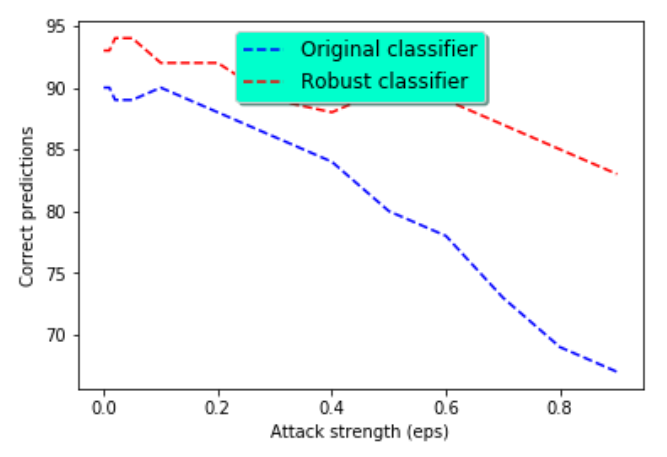
\includegraphics[width=0.9\linewidth,height=50mm]{images/adversarial_training_1.png}
		\caption{$MCAE_{lrc}$}
        \label{fig:normal_vs_robust_f1}
	\end{subfigure}
	\begin{subfigure}{0.48\linewidth}
		\centering
		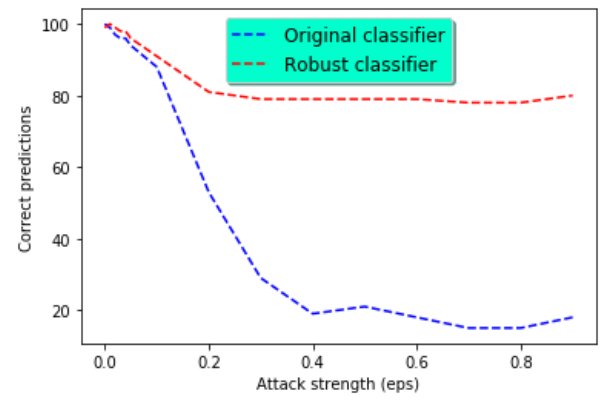
\includegraphics[width=0.9\linewidth,height=50mm]{images/adversarial_training_2.png}
		\caption{$MCAE_{slr}$}
        \label{fig:normal_vs_robust_f2}
	\end{subfigure}
	\caption{Performance comparison: original vs.  robust classifier w.r.t  different \textit{eps} values} 
	\label{fig:normal_vs_robust_models}
\end{figure*}

\begin{table}[h]
    \centering
    \caption{Values of $\hat{\rho}_{\text {adv }}^{\infty}$ for two different networks based on DeepFool and FGSM}
    \begin{tabular}{l|c|c}
        \hline \textbf{Classifier} & \textbf{DeepFool} & \textbf{Fast gradient sign method} \\ \hline $F_1$ & 0.29 & 0.09 \\ \hline 
        $F_2$ & 0.21 & 0.05 \\
        \hline
    \end{tabular}
    \label{tab:robustness_result}
\end{table}

\hspace*{3.5mm} In particular, $F_1$ shows robustness even when $\epsilon$ upto 0.4, giving upto 85\% accuracy, whereas $F_1$ shows very fragile performance, giving drastic reduction of the accuracy of about 25\%. \Cref{tab:robustness_result} reports the $\ell_{\infty}$ robustness to adversarial perturbations for four different networks based on DeepFool and FGSM with $90 \%$ of misclassification.  \Cref{tab:robustness_result} shows the ERM scores for both classifiers. Since a higher ERM value indicates a more robust classifier, it is clear that $F_1$ shows more robust against AEx generated by both DeepFool and FGSM attacks. 

\begin{table}
    \centering
    \caption{Comparison between the average untargeted CLEVER score and distortion found by FGSM and DeepFool untargeted attacks}
    \begin{tabular}{l|l|l|l|l|}
    \cline {2-5} \multicolumn{1}{c|} {} & \multicolumn{2}{c|} {\text {DeepFool}} & \multicolumn{2}{c|} {\text {FGSM}} \\
    \hline Classifier & $\ell_{2}$ & $\ell_{\infty}$ & $\ell_{2}$ & $\ell_{\infty}$ \\
    \hline $F_1$ & 89.25 & 87.54 & 89.25 & 87.54 \\
    \hline $F_2$ & 83.21 & 82.32 & 86.16 & 85.37 \\
    \hline
    \end{tabular}
    \label{tab:my_label}
\end{table}

\iffalse
\begin{table*}[htp!]
	\centering
	\caption{Results of distinguishing ID and OOD (full) test sets of two different classifiers covering detection error, FPR, AUROC, AUPR In~(AUPRI), and AUPR Out~(AUPRO)} 
	\scriptsize{
	\vspace{-4mm}
	\begin{tabular}{llllllllllll}
		&\multicolumn{5}{c}{\bfseries{$MCAE_{lrc}$}} && \multicolumn{5}{c}{\bfseries{$MCAE_{slr}$}} \\	
		\cmidrule{2-6}\cmidrule{8-12}   
		\textbf{Attack type}&\textbf{$\ell_{2}$} & \textbf{$\ell_{\infty}$} & \textbf{AUROC$\uparrow$} & \textbf{AUPRI$\uparrow$} & \textbf{AUPRO$\uparrow$}
		&& \textbf{FPR$\downarrow$} & \textbf{DE$\downarrow$} & \textbf{AUROC$\uparrow$} & \textbf{AUPRI$\uparrow$} & \textbf{AUPRO$\uparrow$}\\
		\hline
		\multirow{1}{*}{{DeepFool}} & 100 & 0.87 & 0.87 & 0.87 & 0.87 && 0.70 & 0.70 & 0.70 & 0.83 & 0.87\\
		\hline
		\multirow{1}{*}{{FGSM}} & 100 & 0.67 & 0.66 & 0.66 & 0.87 && 0.58 & 0.60 & 0.59 & 0.60 & 0.59\\
		\hline
	\end{tabular}}
	\vspace{-2mm}
	\label{Table:OOD_result_2}
\end{table*}
\fi 

\hspace*{3.5mm} On the other hand, in \cref{tab:my_label}, we provide the comparison between the average untargeted CLEVER scores and distortion based on the FGSM and DeepFool untargeted attacks. As expected, CLEVER is smaller than the distortions of adversarial samples in most cases. 
Since CLEVER is independent of attack algorithms, the reported CLEVER scores roughly indicate the distortion of the best possible attack w.r.t a specific $\ell_{p}$ distortion. In the same line, the CLEVER scores can be considered as a security checkpoint for unseen attacks. Since we observe substantial gaps in distortion between the CLEVER score and the considered attack algorithms~(e.g., DeepFool or FGSM), it suggest the existence of a more effective attack that can close the gap~\cite{weng2018evaluating}.

\subsection{OOD detection performance}
Our approach based on~\cite{OOD19}, can distinguish between in- and OOD samples moderately. As shown in \cref{fig:max_soft_score}, there is moderately less overlap between OOD samples and ID samples on the dataset. The relationship between the discrepancy loss and the DE on the test samples are shown in \cref{Table:OOD_result_2}. As observed the discrepancy loss of ID samples is smaller than OOD samples in most of the settings. It can also be noticed that the DE is lower when the difference between the discrepancy loss of ID and OOD samples is larger, which means ID and OOD samples can be separated by the divergence between the two classifiers’ outputs. As demonstrated, more test sample help decrease both DE, ID/OOD discrepancy losses, upto a certain point. For example, when we evaluate the models on 1,800 samples, all the 3 metrics increased, which is probably because of more discrepancy loss. 

\iffalse
\begin{figure}
    \centering
    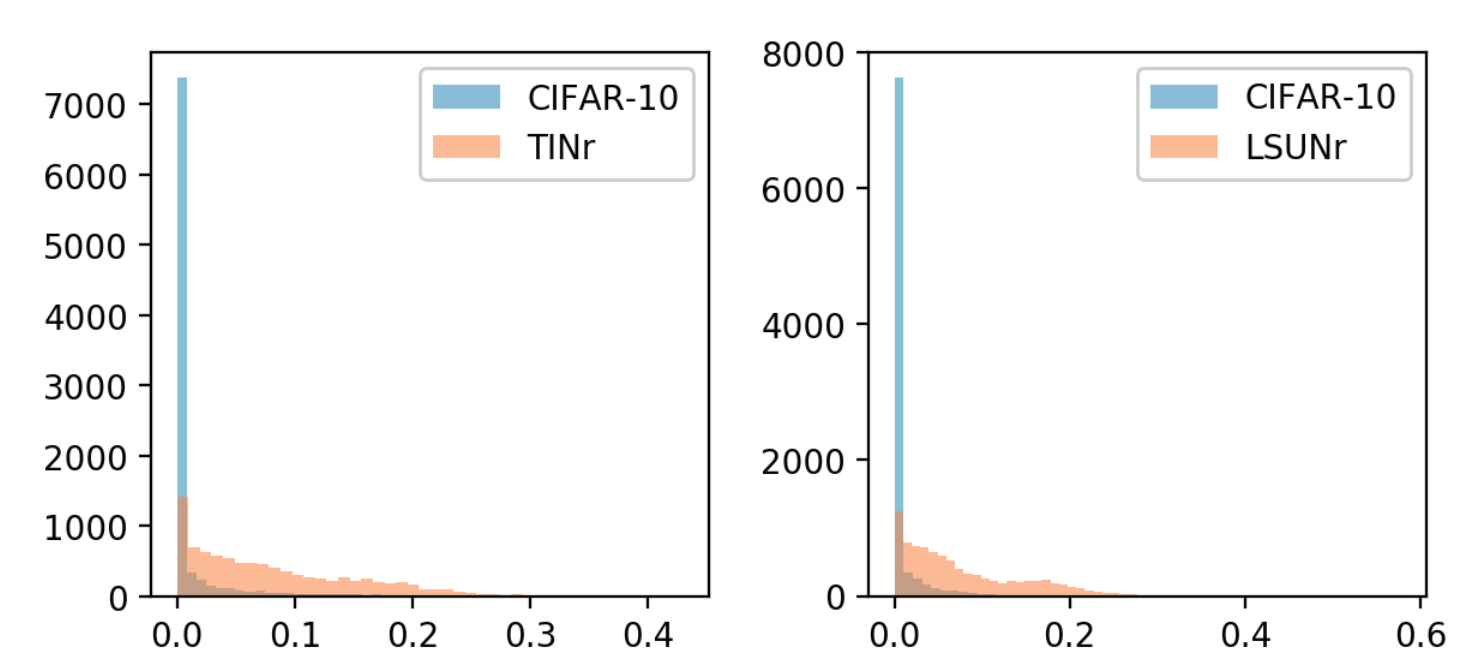
\includegraphics[width=\textwidth,height=60mm]{images/dis_loss.png}
    \caption{Histogram of the discrepancy loss between two classifiers trained on ID samples}
    \label{fig:hist_discre_loss}
\end{figure}
\fi 

%, indicating that our method separates ID and OOD samples very well. Another merit of our method is that we can use a simple
%threshold 1:0 to separate ID and OOD samples as shown in
%Fig. 5a.

\iffalse
\begin{figure}
    \centering
    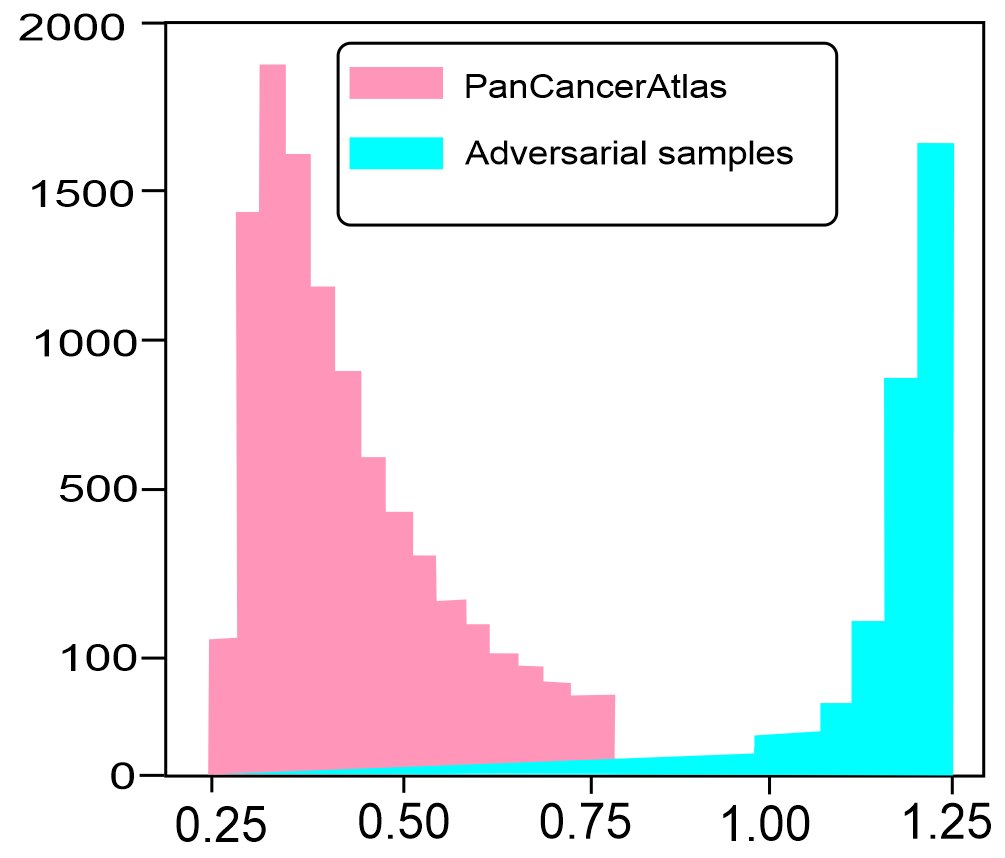
\includegraphics[width=0.5\textwidth,height=60mm]{images/ood_detection.png}
    \caption{Histogram of ID and OOD detection scores}
    \label{fig:ood_detection}
\end{figure}
\fi 

\begin{table*}[htp!]
	\centering
	\caption{Results of distinguishing ID and OOD (full) test sets of two different classifiers covering detection error, FPR, AUROC, AUPR In~(AUPRI), and AUPR Out~(AUPRO)} 
	\scriptsize{
	\vspace{-4mm}
	\begin{tabular}{llllllllllll}
		&\multicolumn{5}{c}{\bfseries{$F_1$}} && \multicolumn{5}{c}{\bfseries{$F_2$}} \\	
		\cmidrule{2-6}\cmidrule{8-12}   
		\textbf{Modality}&\textbf{FPR$\downarrow$} & \textbf{DE$\downarrow$} & \textbf{AUROC$\uparrow$} & \textbf{AUPRI$\uparrow$} & \textbf{AUPRO$\uparrow$}
		&& \textbf{FPR$\downarrow$} & \textbf{DE$\downarrow$} & \textbf{AUROC$\uparrow$} & \textbf{AUPRI$\uparrow$} & \textbf{AUPRO$\uparrow$}\\
		\hline
		\multirow{1}{*}{{GE}} & 100 & 0.87 & 0.87 & 0.87 & 0.87 && 0.70 & 0.70 & 0.70 & 0.83 & 0.87\\
		\hline
		\multirow{1}{*}{{miRNA}} & 100 & 0.67 & 0.66 & 0.66 & 0.87 && 0.58 & 0.60 & 0.59 & 0.60 & 0.59\\
		\hline
		\multirow{1}{*}{{CNV}} & 100 & 0.87 & 0.87 & 0.87 & 0.66 && 0.70 & 0.70 & 0.70 & 0.60 & 0.59\\
		\hline
		\multirow{1}{*}{{GE+miRNA}} & 100 & 0.67 & 0.66 & 0.66 & 0.66 && 0.58 & 0.60 & 0.59 & 0.60 & 0.59\\
		\hline
		\multirow{1}{*}{{GE+CNV}} & 100 & 0.87 & 0.87 & 0.87 & 0.66 && 0.70 & 0.70 & 0.70 & 0.60 & 0.59\\
		\hline
		\multirow{1}{*}{{miRNA+CNV}} & 100 & 0.67 & 0.66 & 0.66 & 0.66 && 0.58 & 0.60 & 0.59 & 0.60 & 0.59\\
		\hline
		\multirow{1}{*}{{GE+miRNA+CNV}} & 100 & 0.87 & 0.87 & 0.87 & 0.66 && 0.70 & 0.70 & 0.70 & 0.60 & 0.59\\
		\hline
	\end{tabular}}
	\vspace{-2mm}
	\label{Table:OOD_result_2}
\end{table*}

\hspace*{3.5mm} Besides, we observe moderately high disagreement, w.r.t between two classifiers' outputs based on unlabeled ID and OOD samples after training the network on labeled ID samples in a supervised way. The histogram of the classifier's maximum softmax scores in \cref{fig:max_soft_scores_and_de_scores} shows that the distribution of the score moderately different w.r.t whether a sample is ID or OOD after the fine-tuning: $p_{1k}$ and $p_{2k}$ denote the probability distribution for class $k$. The discrepancy loss makes OOD sample's maximum $p_{1k}$ close to $1/K$ and maximum $p_{2k}$ close to 1. On the other hand, ID samples' $p_{1k}$ mostly similar to $p_{2k}$, which is based on the support outlined in \cref{eq:ood_join_loss}.

\iffalse
\begin{figure}
    \centering
    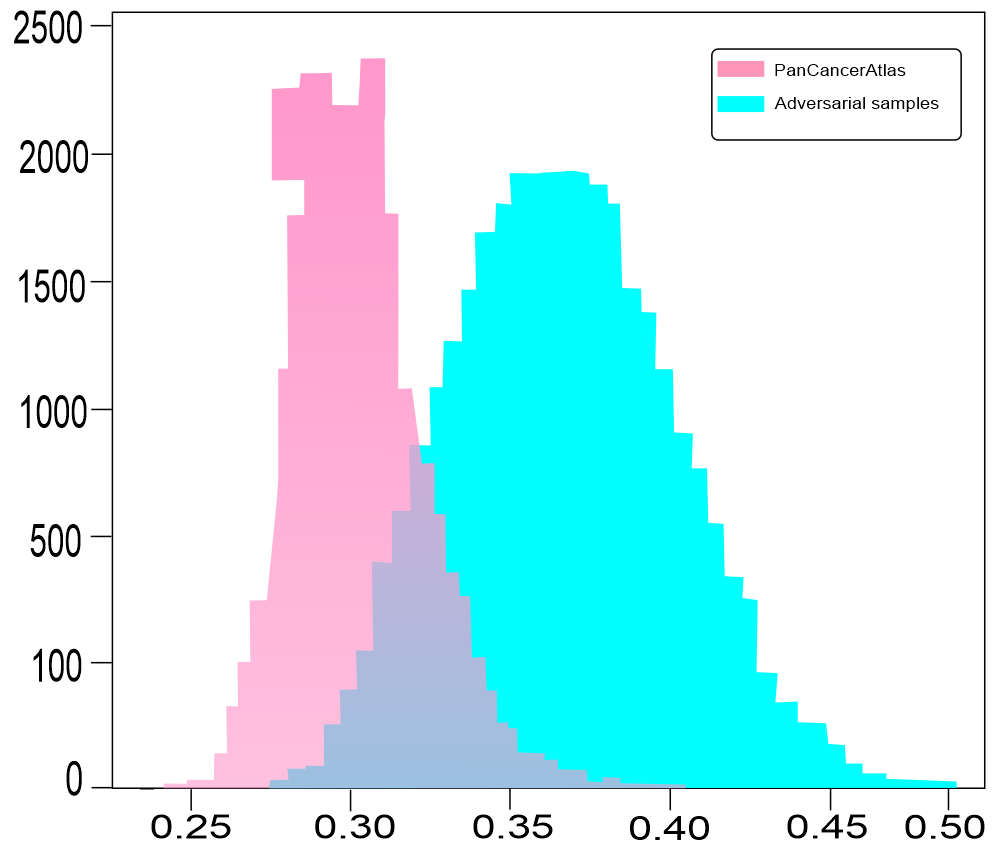
\includegraphics[width=\textwidth,height=60mm]{images/hist_max_softmax.png}
    \caption{Histogram of the two classifier's maximum softmax scores after the fine-tuning}
    \label{fig:hist_softmax_scores}
\end{figure}
\fi 

\begin{figure*}[h]
	\centering
	\begin{subfigure}{.48\linewidth}
		\centering
		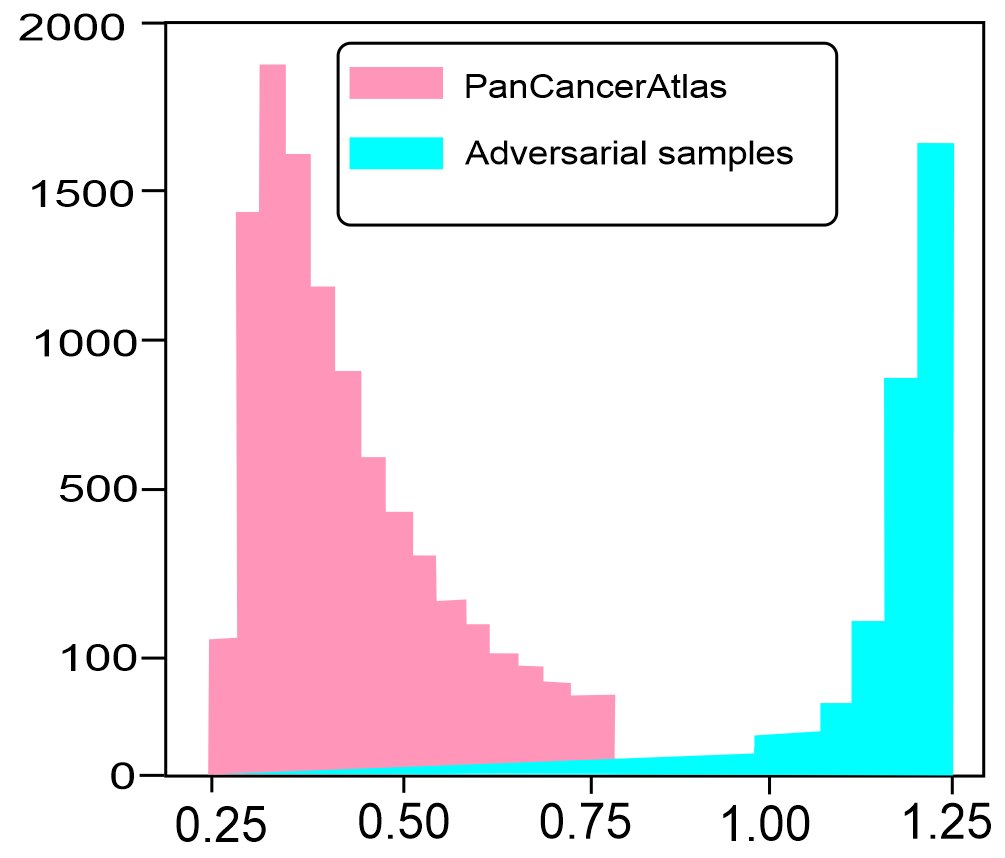
\includegraphics[width=0.9\linewidth,height=50mm]{images/ood_detection.png}
		\caption{Histogram of maximum softmax scores}
        \label{fig:max_soft_score}
	\end{subfigure}
	\begin{subfigure}{0.48\linewidth}
		\centering
		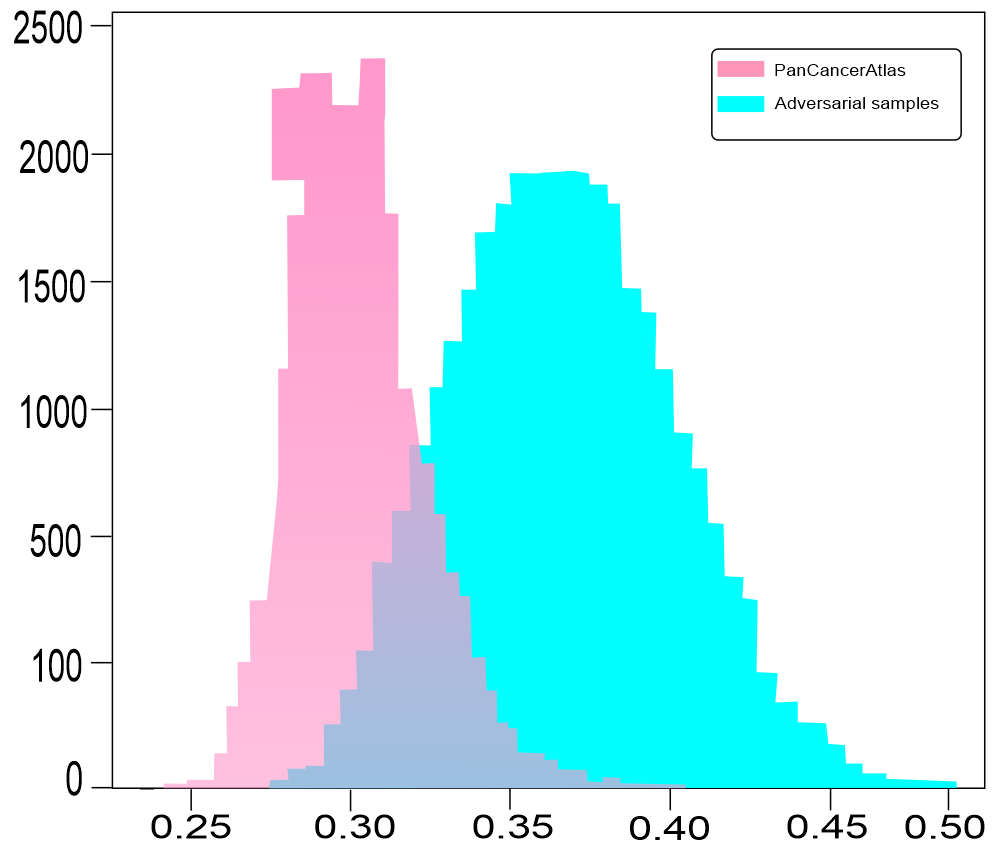
\includegraphics[width=0.9\linewidth,height=50mm]{images/hist_max_softmax.png}
		\caption{Histogram of ID and OOD detection scores}
		\label{fig:id_ood_de_scores}
	\end{subfigure}
	\caption{Histogram of the maximum softmax and ID/OOD detection scores of the classifiers} 
	\label{fig:max_soft_scores_and_de_scores}
\end{figure*}

\hspace*{3.5mm} As seen, the discrepancy loss of ID samples is smaller than OOD samples in all settings. The DE is lower when the difference between the discrepancy loss of ID and OOD samples is larger, which means ID and OOD samples can be separated by the divergence between the two classifiers' output. Since this method needs to fine-tune the classifiers in order to detect the OOD samples, the decision boundary changed slightly. Eventually, we see a significant drop of classification accuracy~(by 8\%) compared to original accuracy we observed in \cref{chapter:xai}. We ca observe that GE and miRNA are more sensitive to making changes, which reflect in the GE, miRNA, GE+miRNA modalities too. 

%This problem could be solved by using the original classifier to classify ID samples with some runtime increase and it is still much more acceptable than ELOC [26] using an ensemble of five models which needs more runtime and computing resources.

%\section{Discussion} \label{chapter_6:discussion}

\section{Chapter Summary} \label{chapter_6:conclusion}
In this chapter, discussed how to improve the adversarial robustness of an explainable model. We apply different types of adversarial attacks on our model by generating AEx with content moderation attack by introducing noise, generating AEx as OOD. Then we impose both proactive and reactive counter measurements before assessing the robustness against each scenario. 
For detecting OOD, we trained two different classifiers to detect OOD samples that are far from the support of the ID samples. However, considering the scope of this thesis, we try to limit the discussion within simple methods. In future, we intend to focus more employ not so complicated and sophisticated counter-measurements. 

%Our method does not require labeled OOD samples to train the neural network. 
%We extensively evaluated our method not only on OOD detection benchmarks, but also on real-world simulation datasets. Our method significantly outperformed the current state-of-the-art methods on different DNN architectures across various in and out-of-distribution dataset pairs. 

\hspace*{3.5mm} In the previous chapter, we have seen that explaining the predictions with plots and charts are good for exploration and discovery, but interpreting them for the first time may be very difficult, especially for the non-domain experts/users. This is also applicable for the patients. Therefore, in the next chapter, we provide more human-understandable and model-agnostic explanations based on IF-THEN rules. Using anchors, we will see how to explain individual predictions of our black-box models by finding a decision rule that ``Rule-matrix" and ``Bayesian Rule List" the prediction sufficiently. 
%In \cref{chapter:nsr}, we will see how to combine model predictions, interpretation, and reasoning to provide more fair rules. 

